
\section{Results of Experiment 1: Pointing Correction Model}
In this section, we present the results obtained from experiment $1$ introduced in section \ref{sec:exp1}.
Prior to presenting the results, we provide a reminder of the RMS ratio measure \eqref{eq:mean_rms_compared}, which we frequently used in this section.
We used this measure to compare the current pointing model to the machine learning model, and a value less than $1$ indicates an improvement of the current model. \\

Table \ref{tab:results_minval_val_test_days_04_n230} presents the validation and test RMS ratios for all folds of the NFLASH230 model in case 1 and case 2.
Recall that models were trained with different numbers of features $k$, and these results are from the model with the best performance on the validation set (can be different $k$ for each fold).
The results show that the model's performance on the validation set is very good in both case 1 and 2.
However, this does not generalize well to the test set, with the performance on the test set for case 1 being significantly worse than the current model for all folds.
In contrast, for case 2, the performance on the test set is better than the current model for most of the folds.
Table \ref{tab:results_minval_val_test_days_04_all} presents the same results for the model predicting the offsets of all instruments.
This model exhibits similar trends, although its performance on the test set is not as good as the NFLASH230 model.\\

\begin{table}[!htbp]
    \centering
    \caption[NFLASH230 pointing correction model results on each fold]{
    Validation and test performance measured in RMS ratio \eqref{eq:rms_compared} in case 1 and 2 (see Figure \ref{fig:datasplit_cases}) for the pointing correction model trained on NFLASH230 data.
    The performance is given for the model complexity $k$ that yields the best results on the validation data for the given fold.}
    \begin{tabular}{lccccc}
        \toprule
        & & \multicolumn{2}{c}{Case 1 RMS ratio} & \multicolumn{2}{c}{Case 2 RMS ratio} \\
        \cmidrule{3-4} \cmidrule{5-6}
        Target & Fold & Validation & Test &  Validation &  Test \\
        \midrule
        \multirow{6}{*}{Azimuth} & 1 &  0.848 &       1.188 &      0.846 &       1.043 \\
                            & 2 &  0.841 &       1.427 &      0.870 &       0.962 \\
                            & 3 &  0.840 &       1.462 &      0.923 &       0.882 \\
                            & 4 &  0.837 &       1.266 &      0.873 &       0.989 \\
                            & 5 &  0.846 &       1.242 &      0.879 &       0.944 \\
                            & 6 &  0.837 &       1.318 &      0.907 &       0.930 \\
        \hline
        \multirow{6}{*}{Elevation} & 1 &  0.835 &       1.173 &      0.887 &       1.030 \\
                            & 2 &  0.831 &       1.188 &      0.889 &       0.973 \\
                            & 3 &  0.831 &       1.204 &      0.886 &       1.025 \\
                            & 4 &  0.812 &       1.198 &      0.826 &       0.844 \\
                            & 5 &  0.815 &       1.166 &      0.802 &       0.870 \\
                            & 6 &  0.810 &       1.262 &      0.825 &       0.906 \\
        \bottomrule
    \end{tabular}
    \label{tab:results_minval_val_test_days_04_n230}
\end{table}

\newpage 
\begin{table}[!htbp]
    \centering
    \caption[All instruments pointing correction model results on each fold]{
    Validation and test performance measured in RMS ratio \eqref{eq:rms_compared} in case 1 and 2 (see Figure \ref{fig:datasplit_cases}) for the pointing correction model trained on all data.
    The performance is given for the model complexity $k$ that yields the best results on the validation data for the given fold.}
    \begin{tabular}{lccccc}
        \toprule
        & & \multicolumn{2}{c}{Case 1 RMS ratio} & \multicolumn{2}{c}{Case 2 RMS ratio} \\
        \cmidrule{3-4} \cmidrule{5-6}
        Target & Fold & Validation & Test &  Validation &  Test \\
        \midrule
        \multirow{6}{*}{Azimuth} & 1 &  0.870 &       1.642 &      0.881 &       1.233 \\
                            & 2 &  0.861 &       1.626 &      0.971 &       0.928 \\
                            & 3 &  0.876 &       1.784 &      0.897 &       1.016 \\
                            & 4 &  0.866 &       1.613 &      0.938 &       0.950 \\
                            & 5 &  0.862 &       1.935 &      0.927 &       0.942 \\
                            & 6 &  0.874 &       1.779 &      0.923 &       1.027 \\
                            \hline
        \multirow{6}{*}{Elevation} & 1 &  0.832 &       1.193 &      0.948 &       0.965 \\
                            & 2 &  0.831 &       1.141 &      0.924 &       1.051 \\
                            & 3 &  0.824 &       1.129 &      0.929 &       1.094 \\
                            & 4 &  0.816 &       1.172 &      0.822 &       0.922 \\
                            & 5 &  0.818 &       1.196 &      0.828 &       0.978 \\
                            & 6 &  0.822 &       1.186 &      0.831 &       0.951 \\
                            \bottomrule
    \end{tabular}
    \label{tab:results_minval_val_test_days_04_all}
\end{table}


In addition to Table \ref{tab:results_minval_val_test_days_04_n230} and Table \ref{tab:results_minval_val_test_days_04_all},
we also evaluated the performance of the NFLASH230 model with different complexities.
Table \ref{tab:results_nflash_days} shows the mean RMS ratio \eqref{eq:mean_rms_compared} on the test set,
and the associated standard deviation for the azimuth and elevation models when using the same number of features $k$ on all folds.
By inspection, we see that the machine learning model does not provide any improvement over the current pointing model for case 1, apart from a slight improvement of an average of $1.8\%$ reduced RMS with a standard deviation of $1.4\%$ for the azimuth model with number of features $k=2$.
However, case 2 shows more promising results.
For azimuth, the best RMS ratio is $0.948$ with a standard deviation of $0.056$, which is an average improvement of $5.2\%$ reduced RMS on all folds, with a standard deviation of $5.6\%$.
The number of features for these results is $k=2$.
Using $k=50$ features shows similar results, with $0.945$ RMS ratio and a standard deviation of $0.073$.\\

For elevation, the best RMS ratio is $0.940$ with a standard deviation of $0.075$, using $k=50$ features.
Table \ref{tab:results_all_days} shows the same results for case 1 and 2, but for the model trained on data from all instruments.
We see the same trends, with case 1 showing no improvement and case 2 showing a slight improvement for azimuth and elevation.
The best RMS ratio for azimuth in case 2 is $0.980$ with a standard deviation of $0.059$, using $k=2$ features.
For elevation, the best model is the one with $k=50$ features, with a RMS ratio of $0.955$ and a standard deviation of $0.029$.
Overall, the elevation models show slightly better results than the azimuth models.
Additionally, the model predicting only NFLASH230 offsets performs better than the model predicting offsets from all instruments. \\


\begin{table}[!htbp]
    \centering
    \caption[NFLASH230 model results for complexity $k$]{%$tmp2022\_clean\_clf\_nflash230\_results\_table$
    Resulting mean RMS ratio \eqref{eq:mean_rms_compared} on unseen test sets in case $1$ and $2$ (see Figure \ref{fig:datasplit_cases}) for the model trained on NFLASH230 data,
    using different number of features $k$ in the model.}
    \begin{tabular}{ccccc c cccc}
        \toprule
        \multicolumn{1}{c}{} & \multicolumn{4}{c}{Case 1} & & \multicolumn{4}{c}{Case 2} \\
        \cmidrule(lr){2-5} \cmidrule(lr){7-10}
        \multicolumn{1}{c}{} & \multicolumn{2}{c}{Azimuth} & \multicolumn{2}{c}{Elevation} & & \multicolumn{2}{c}{Azimuth} & \multicolumn{2}{c}{Elevation} \\ 
        \cmidrule(lr){2-5} \cmidrule(lr){7-10}
        k & Mean & STD & Mean & STD & & Mean & STD & Mean & STD \\ 
        \midrule
         2 &     0.982 &     0.014 &     1.020 &     0.024 &  &  0.948 &     0.056 &     0.972 &     0.081 \\
         5 &     1.366 &     0.077 &     1.198 &     0.034 &  &  0.983 &     0.142 &     0.953 &     0.097 \\
        10 &     1.383 &     0.087 &     1.155 &     0.047 &  &  0.957 &     0.080 &     0.967 &     0.087 \\
        20 &     1.252 &     0.119 &     1.126 &     0.071 &  &  0.972 &     0.131 &     0.949 &     0.069 \\
        30 &     1.335 &     0.226 &     1.094 &     0.041 &  &  0.963 &     0.093 &     0.959 &     0.077 \\
        40 &     1.146 &     0.036 &     1.058 &     0.020 &  &  0.961 &     0.089 &     0.948 &     0.077 \\
        50 &     1.202 &     0.131 &     1.062 &     0.022 &  &  0.945 &     0.073 &     0.940 &     0.075 \\
        \bottomrule
    \end{tabular}
    \label{tab:results_nflash_days}
\end{table}

\begin{table}[!htbp]
    \centering
    \caption[All instruments model results for complexity $k$]{%$tmp2022\_clean\_clf\_results\_table$
    Resulting mean RMS ratio \eqref{eq:mean_rms_compared} on unseen test sets in case $1$ and $2$ (see Figure \ref{fig:datasplit_cases}) for the model trained on all data,
    using different number of features $k$ in the model.}
    \begin{tabular}{ccccc c cccc}
        \toprule
        \multicolumn{1}{c}{} & \multicolumn{4}{c}{Case 1} & & \multicolumn{4}{c}{Case 2} \\
        \cmidrule(lr){2-5} \cmidrule(lr){7-10}
        \multicolumn{1}{c}{} & \multicolumn{2}{c}{Azimuth} & \multicolumn{2}{c}{Elevation} & & \multicolumn{2}{c}{Azimuth} & \multicolumn{2}{c}{Elevation} \\ 
        \cmidrule(lr){2-5} \cmidrule(lr){7-10}
        k & Mean & STD & Mean & STD & & Mean & STD & Mean & STD \\ 
        \midrule
         2 &     1.007 &     0.003 &     1.232 &     0.055 &  &  0.980 &     0.059 &     0.964 &     0.016 \\
         5 &     1.003 &     0.003 &     1.170 &     0.028 &  &  0.990 &     0.067 &     0.964 &     0.016 \\
        10 &     1.288 &     0.101 &     1.116 &     0.015 &  &  1.001 &     0.102 &     0.979 &     0.059 \\
        20 &     1.580 &     0.082 &     1.121 &     0.023 &  &  1.018 &     0.130 &     0.971 &     0.036 \\
        30 &     1.606 &     0.110 &     1.107 &     0.018 &  &  1.026 &     0.151 &     0.957 &     0.018 \\
        40 &     1.528 &     0.111 &     1.068 &     0.010 &  &  1.026 &     0.137 &     0.973 &     0.044 \\
        50 &     1.758 &     0.121 &     1.061 &     0.027 &  &  1.018 &     0.114 &     0.955 &     0.029 \\
        \bottomrule
    \end{tabular}
    \label{tab:results_all_days}
\end{table}

\newpage

Table \ref{tab:results_minval_days04} presents an unbiased estimate of the performance of this approach,
since we chose the model to use on the test set purely based on performance on the validation set.
It shows the mean RMS ratio for the test set on all folds for both models in Tables \ref{tab:results_minval_val_test_days_04_n230} and \ref{tab:results_minval_val_test_days_04_all}.
The results indicate that there is no improvement over the current pointing model for case 1.
However, for case 2, the model predicting only NFLASH230 offsets shows a small improvement over the current model,
with an RMS ratio of $0.958$ for azimuth and $0.941$ for elevation, both with standard deviations of $0.055$ and $0.079$, respectively.\\

Although the results of case 1 have not shown any improvement over the current pointing model, case 2 has demonstrated potential for improving the pointing accuracy.
However, it is important to note that the test data used in the cross-validation process for case 2 is either before or in the middle of the training and validation sets in time, except for the last fold.
In the last fold, the test set falls after the training and validation in time, and for the NFLASH230 model,
the RMS ratio on this fold was $0.930$ for azimuth and $0.906$ for elevation, which represents a $7.0\%$ and $9.4\%$ improvement, respectively.
In contrast, for all instruments, the RMS ratio was $1.027$ for azimuth and $0.951$ for elevation, representing a $2.7\%$ worse performance for azimuth and a $4.9\%$ improvement for elevation.
This result is the most realistic and unbiased estimate we have on the performance of these models.

For a list of the $50$ features with the greatest mutual information to the target variable, please refer to Table \ref{tab:exp2_top50_features} in Appendix \ref{sec:appendix_a}.


 
Figure \ref{fig:histogram_selected_result_xgb} shows the distribution of NFLASH230 offsets with and without the machine learning model corrections.
These are the distribution of offsets of the unseen test set for the last fold.



\begin{figure}[H]
    \centering
    \begin{subfigure}[t]{\textwidth}
        \centering
        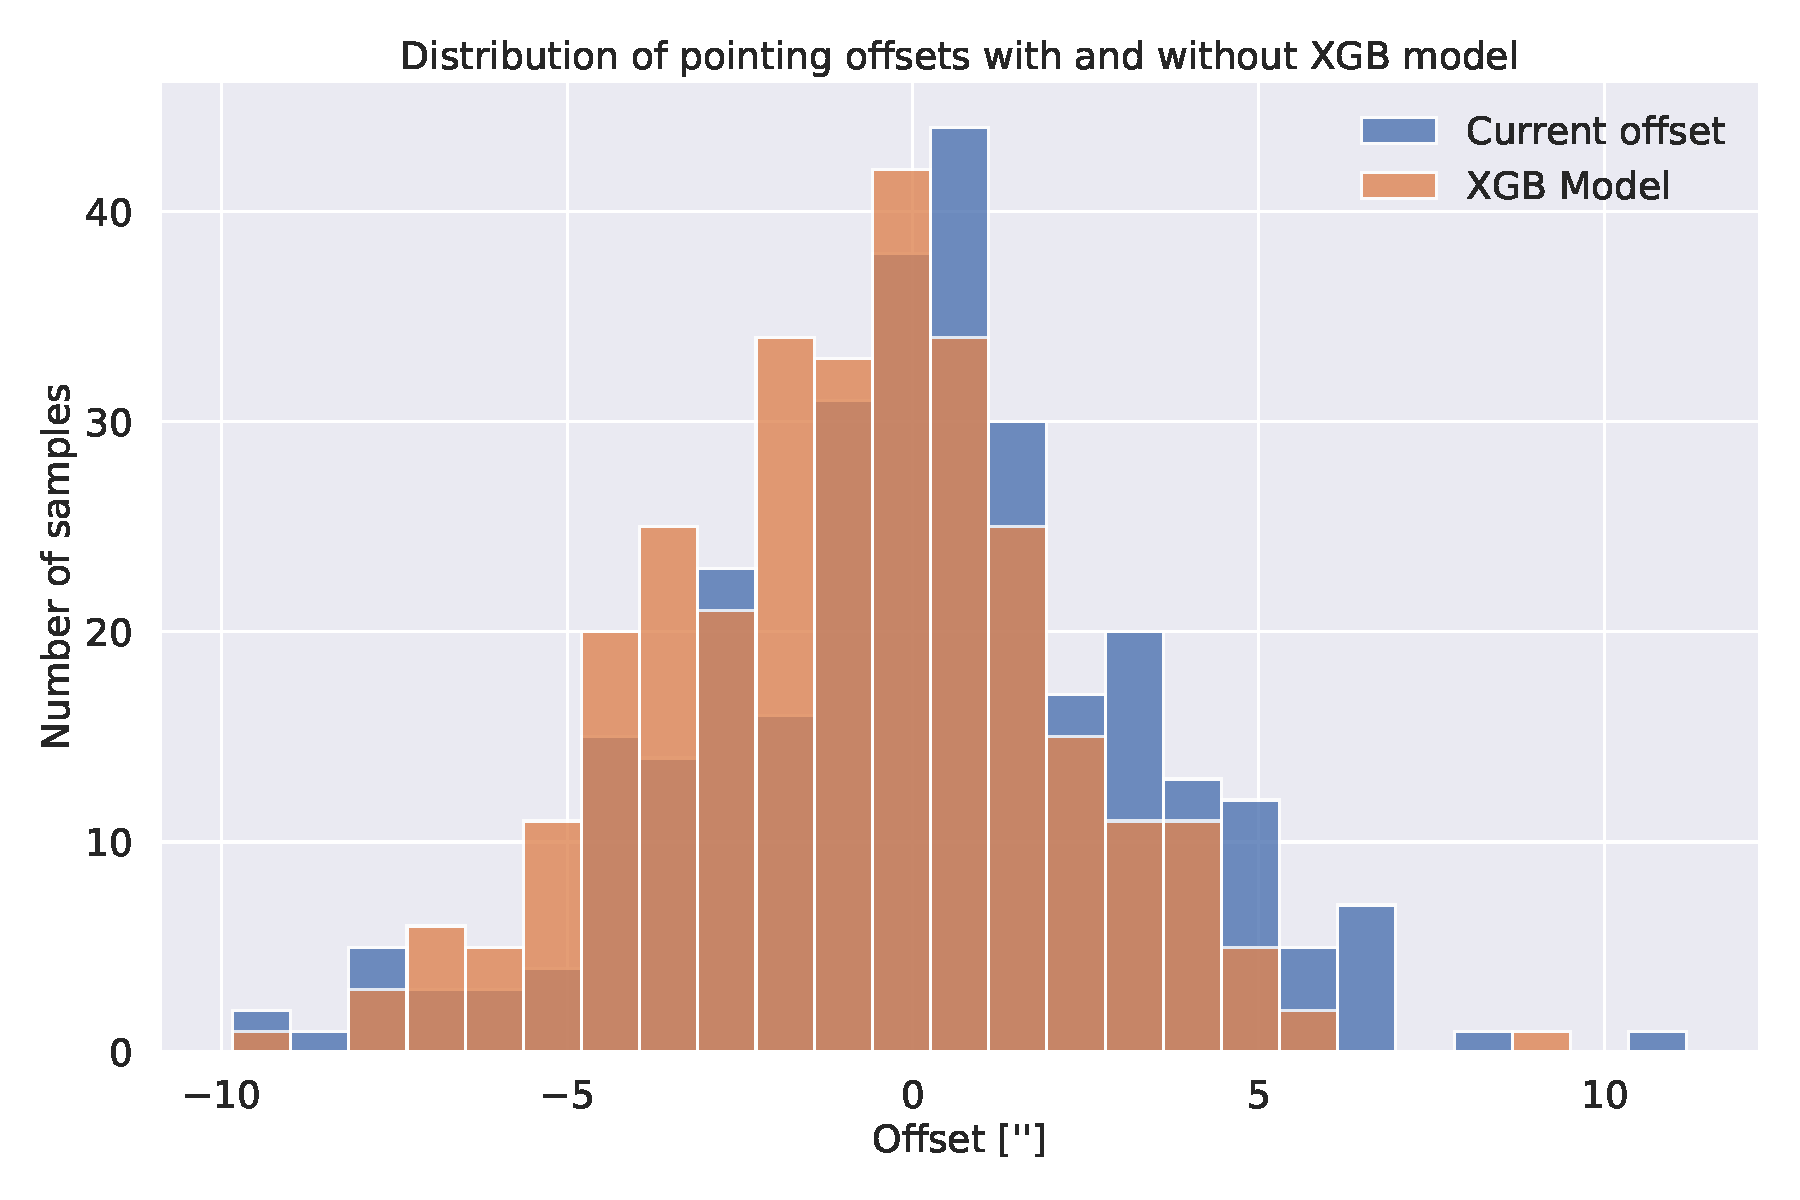
\includegraphics[width=\textwidth]{Results/hist_XGB_ds2_tp5_k30_uncorr_az_test.pdf}
        \caption{The azimuth model, with offsets reduced on the unseen test set by $7.0\%$.}
        \label{subfig:hist_lastfold_nflash230_az}
    \end{subfigure}
    \\
    \begin{subfigure}[t]{\textwidth}
       \centering
       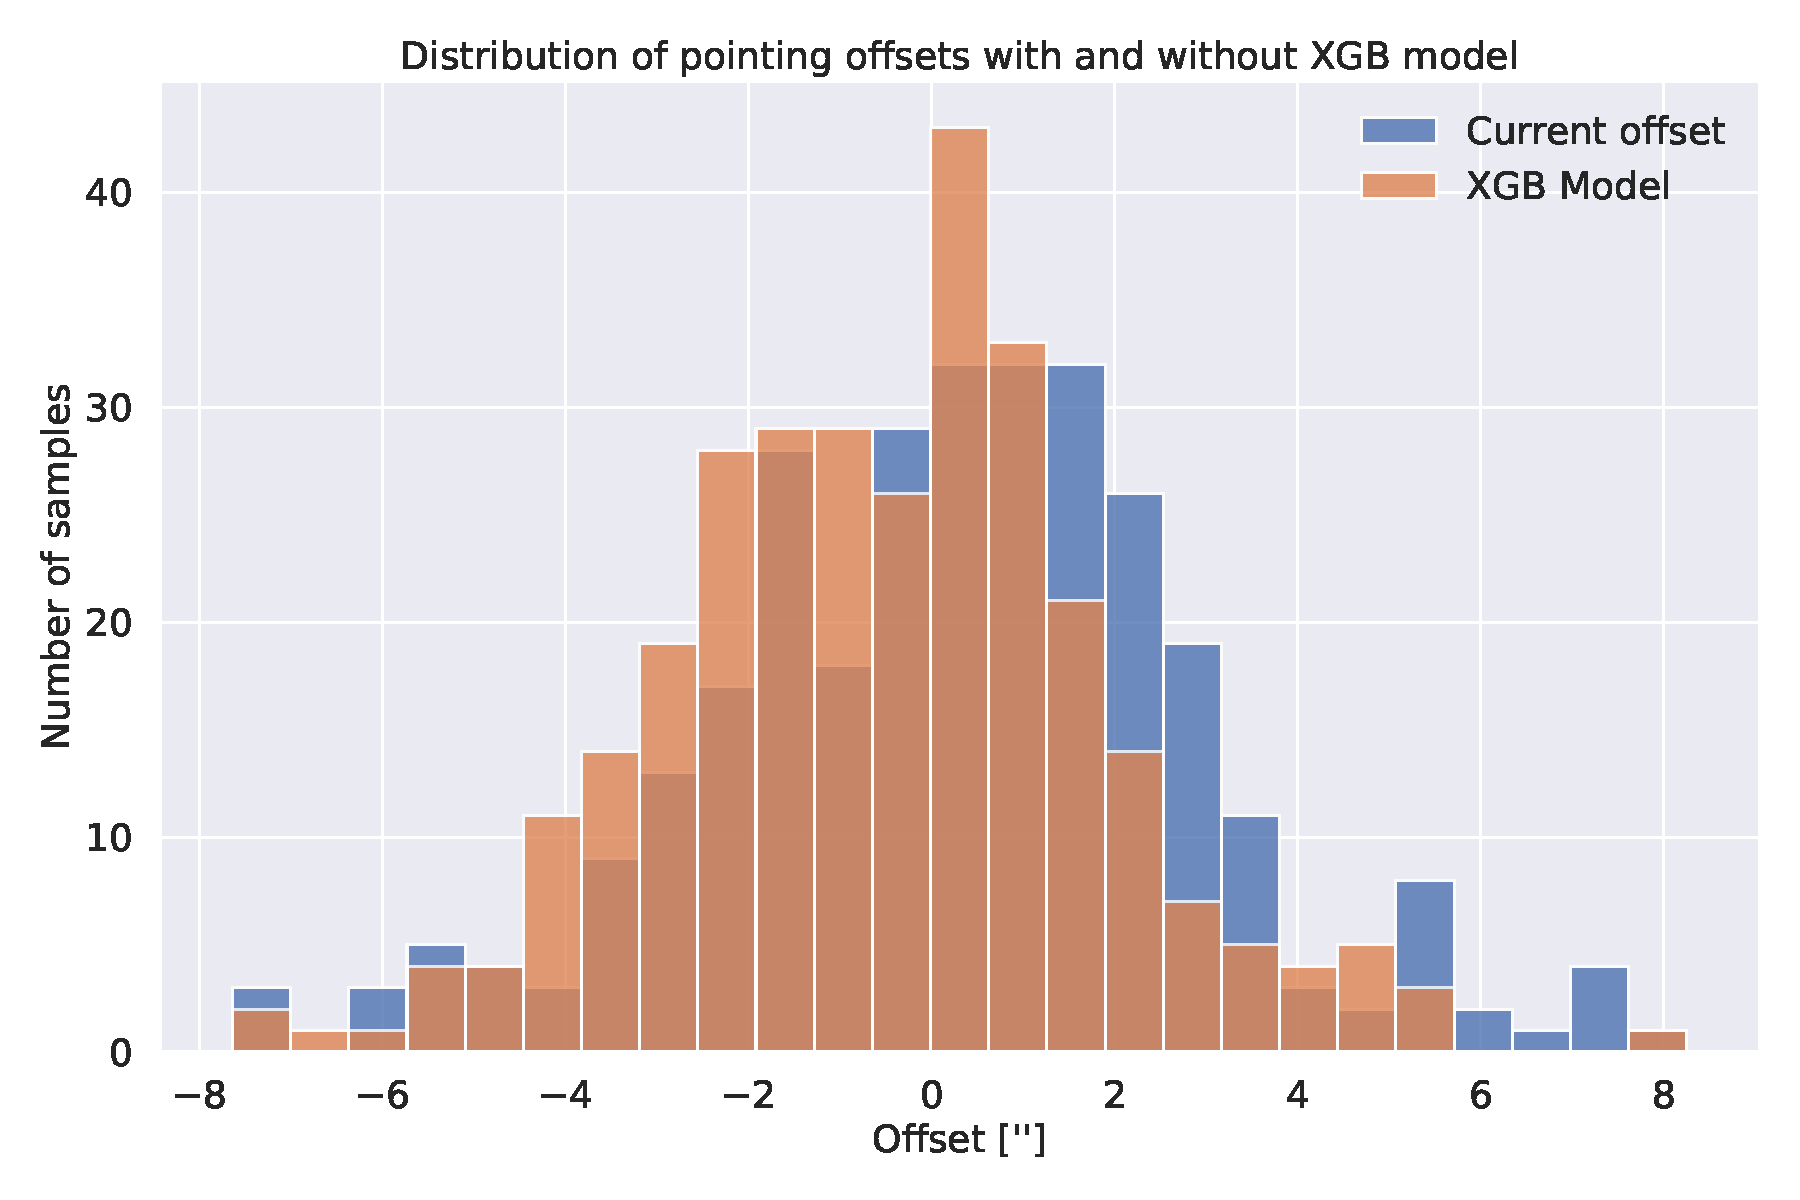
\includegraphics[width=\textwidth]{Results/hist_XGB_ds2_tp5_k40_uncorr_el_test.pdf}
       \caption{The elevation model, with offsets reduced on the unseen test set by $9.4\%$.}
       \label{subfig:hist_lastfold_nflash230_el}
    \end{subfigure}
    \caption[Offset distribution with and without pointing correction model]{Distribution of offsets with and without the NFLASH230 pointing correction model on the unseen test set for the last fold. \textbf{a)} Azimuth model and \textbf{b)} elevation model.}
    \label{fig:histogram_selected_result_xgb}
\end{figure}


Figure \ref{fig:sortpred_selected_result_xgb} show the predicted and observed pointing NFLASH230 offsets for all samples in the unseen test set of the last fold.
We sorted the samples by the true value in ascending order.


\begin{figure}[H]
    \centering
    \begin{subfigure}[t]{\textwidth}
        \centering
        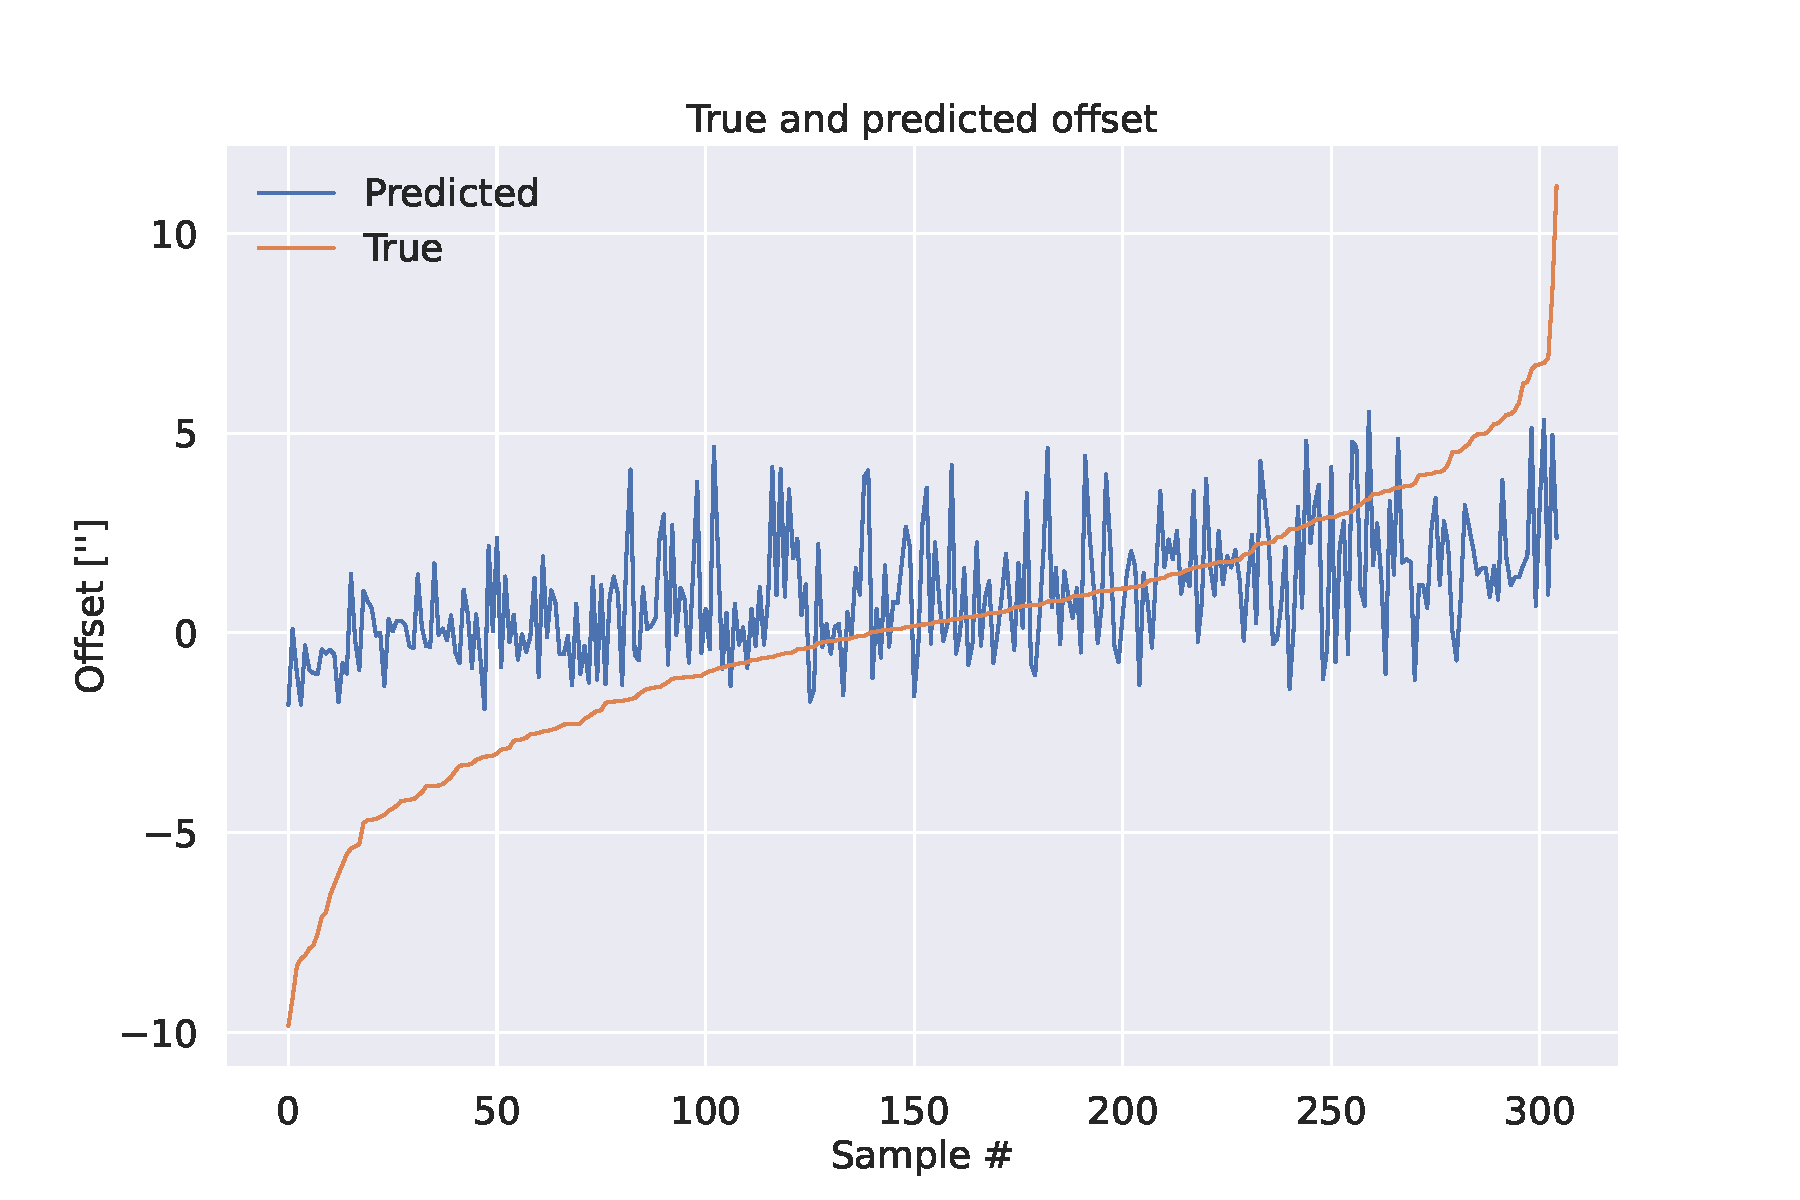
\includegraphics[width=\textwidth]{Results/sortpred_XGB_ds2_tp5_k30_uncorr_az_test.pdf}
        \caption{The azimuth model, with offsets reduced on the unseen test set by $7.0\%$.}
        \label{subfig:sortpred_lastfold_nflash230_az}
    \end{subfigure}
    \\
    \begin{subfigure}[t]{\textwidth}
       \centering
       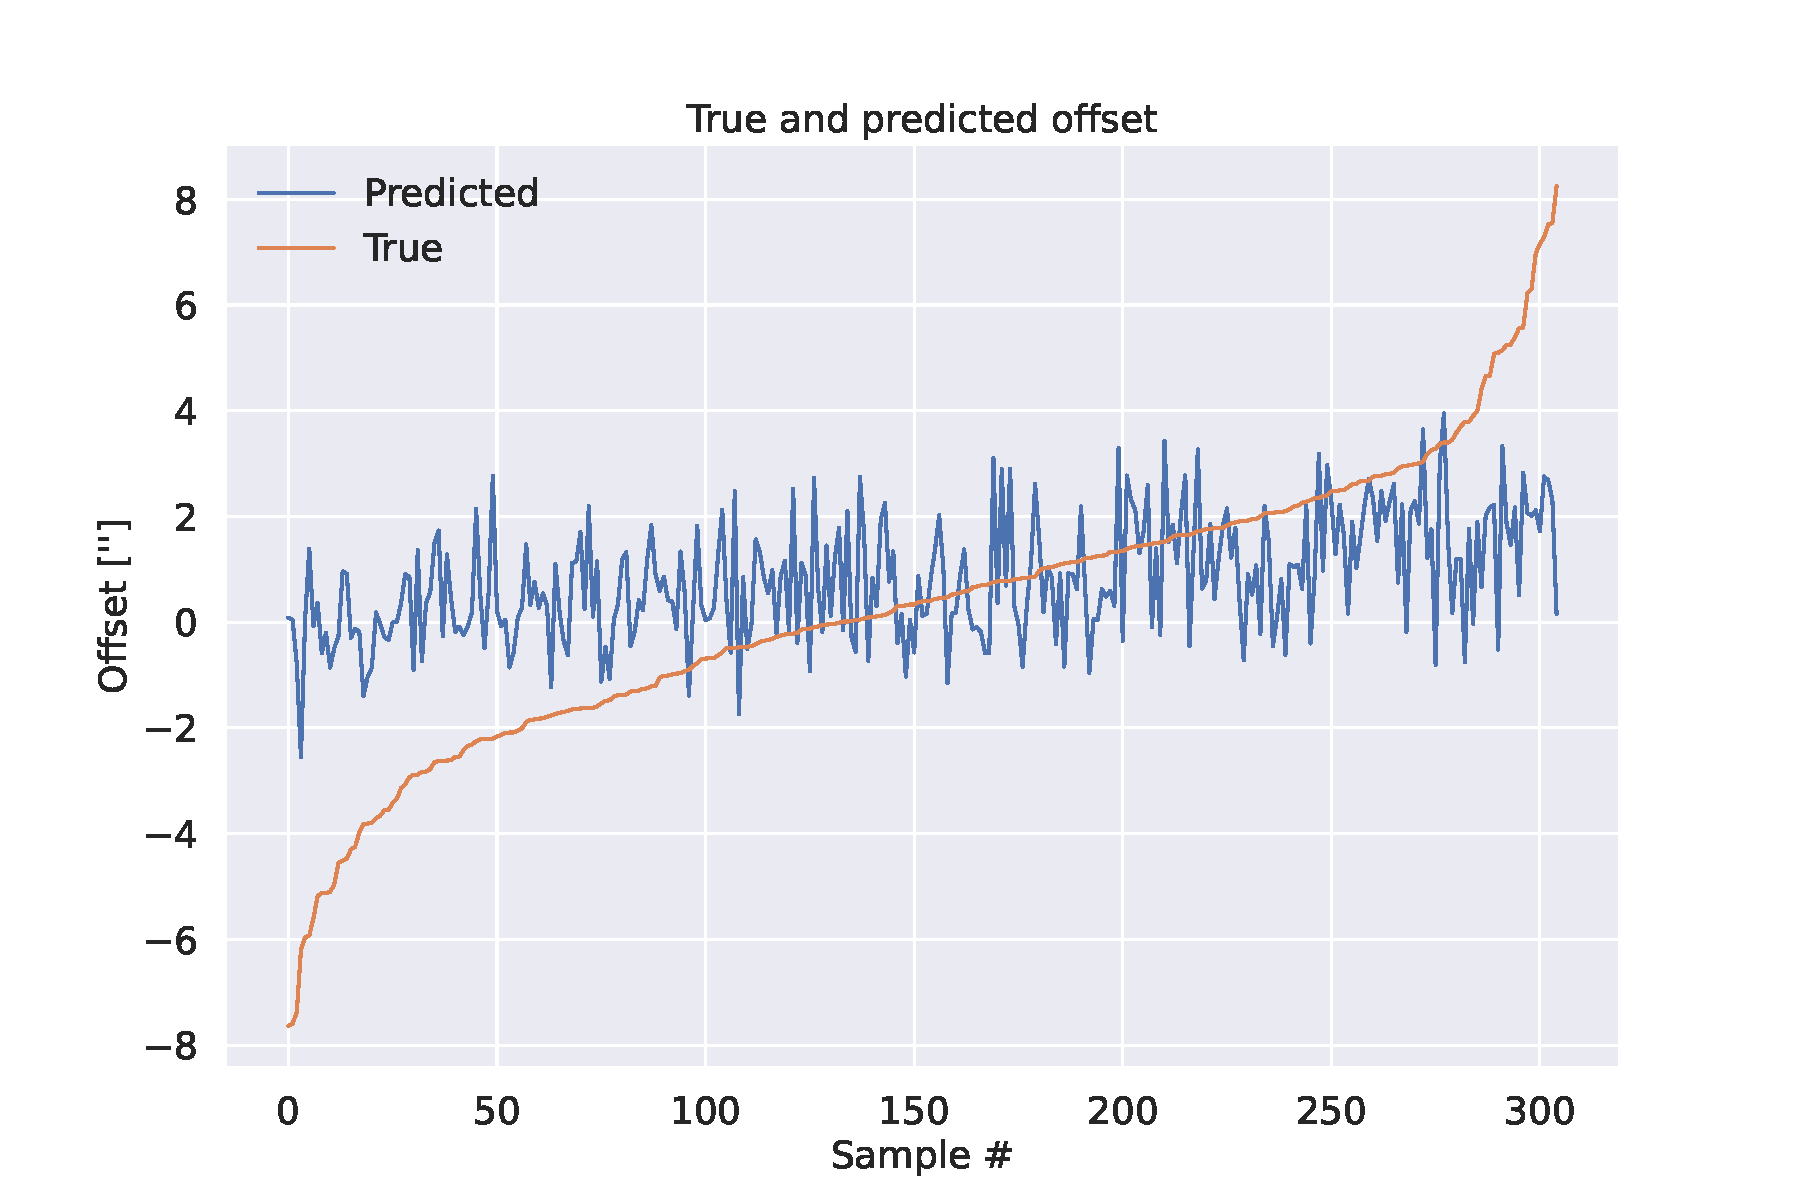
\includegraphics[width=1\textwidth]{Results/sortpred_XGB_ds2_tp5_k40_uncorr_el_test.pdf}
       \caption{The elevation model, with offsets reduced on the unseen test set by $9.4\%$.}
       \label{subfig:sortpred_lastfold_nflash230_el}
    \end{subfigure}
    \caption[Sorted offset prediction and true values]{Offset predictions by the NFLASH230 pointing correction model on the unseen test set for the last fold.
     Predicted and observed values, sorted in ascending order by observed value. \textbf{a)} Azimuth model and \textbf{b)} elevation model.}
    \label{fig:sortpred_selected_result_xgb}
\end{figure}



Figure \ref{fig:sage_lastfold_nflash230_az} show the SAGE values for the NFLASH230 azimuth pointing correction model on the validation set (Figure \ref{subfig:sage_lastfold_nflash230_az_val})
and test set (Figure \ref{subfig:sage_lastfold_nflash230_az_test}).
The same plots for the elevation models are presented in Figure \ref{fig:sage_lastfold_nflash230_el}.

\begin{figure}[H]
    \centering
    \begin{subfigure}[t]{0.92\textwidth}
        \centering
        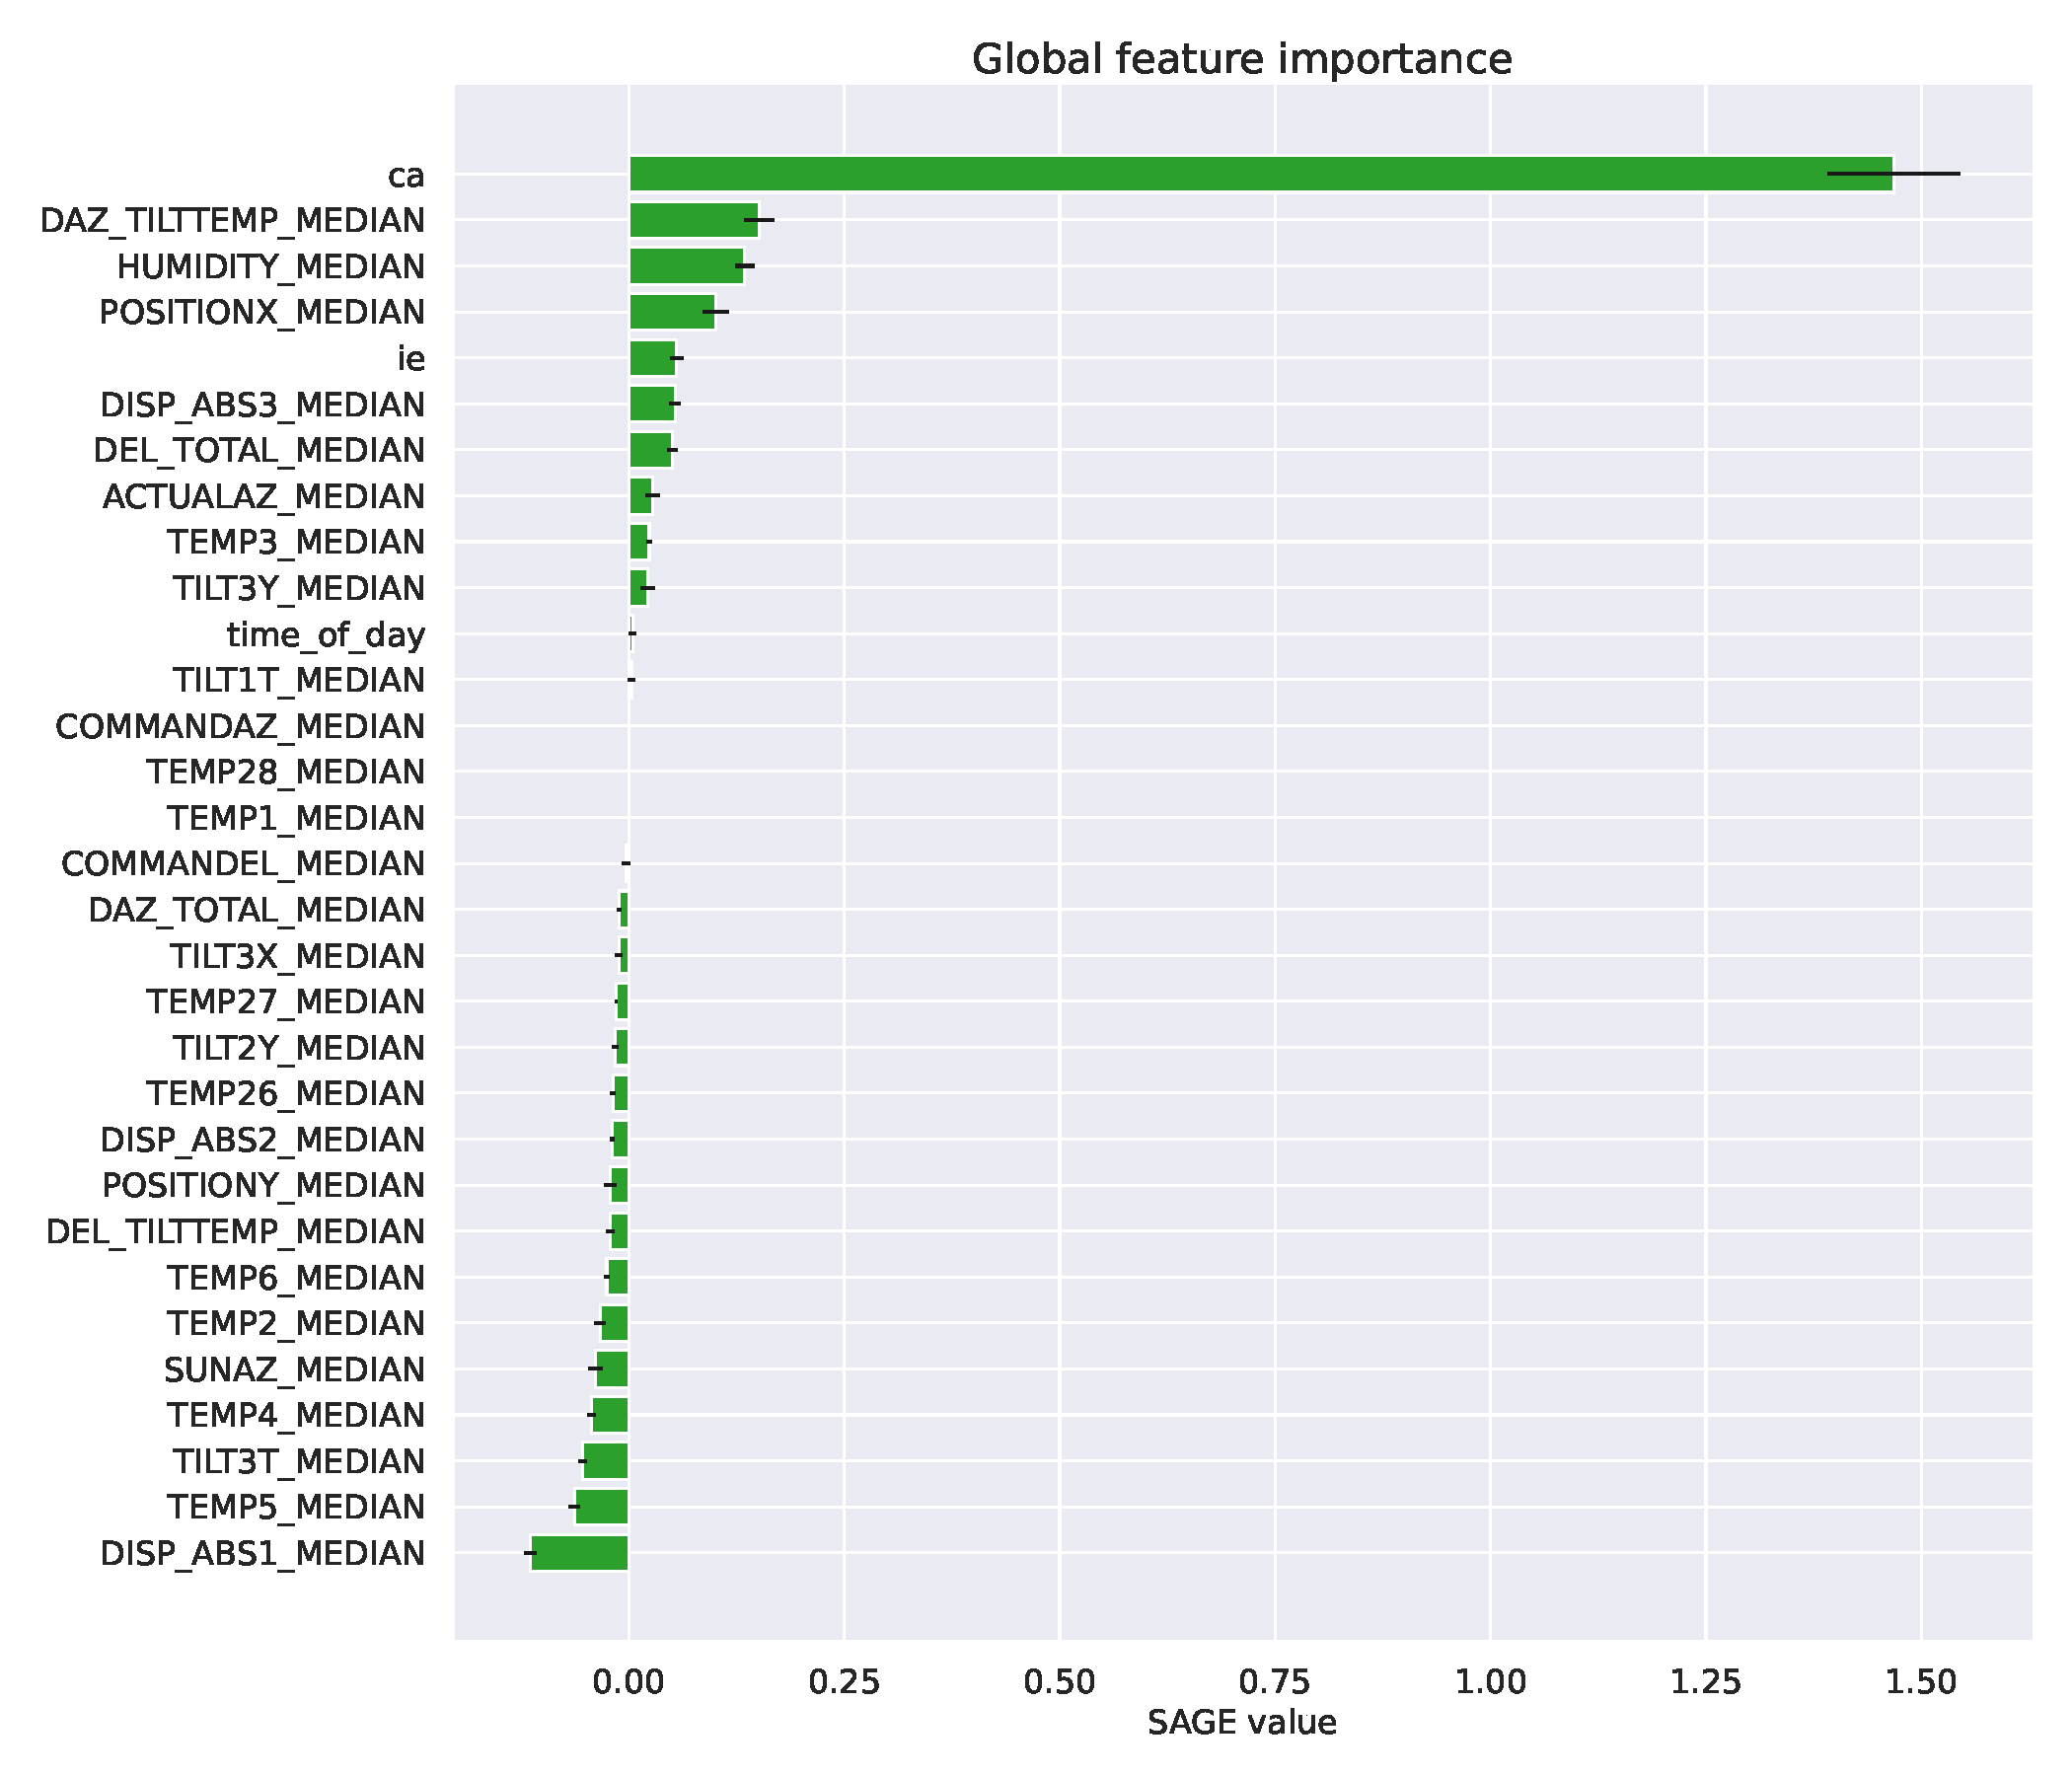
\includegraphics[width=\textwidth]{Results/XGB_ds2_tp5_k30_uncorr_az_val_SAGE.pdf}
        \caption{Validation set}
        \label{subfig:sage_lastfold_nflash230_az_val}
    \end{subfigure}
    \\
    \begin{subfigure}[t]{0.92\textwidth}
       \centering
       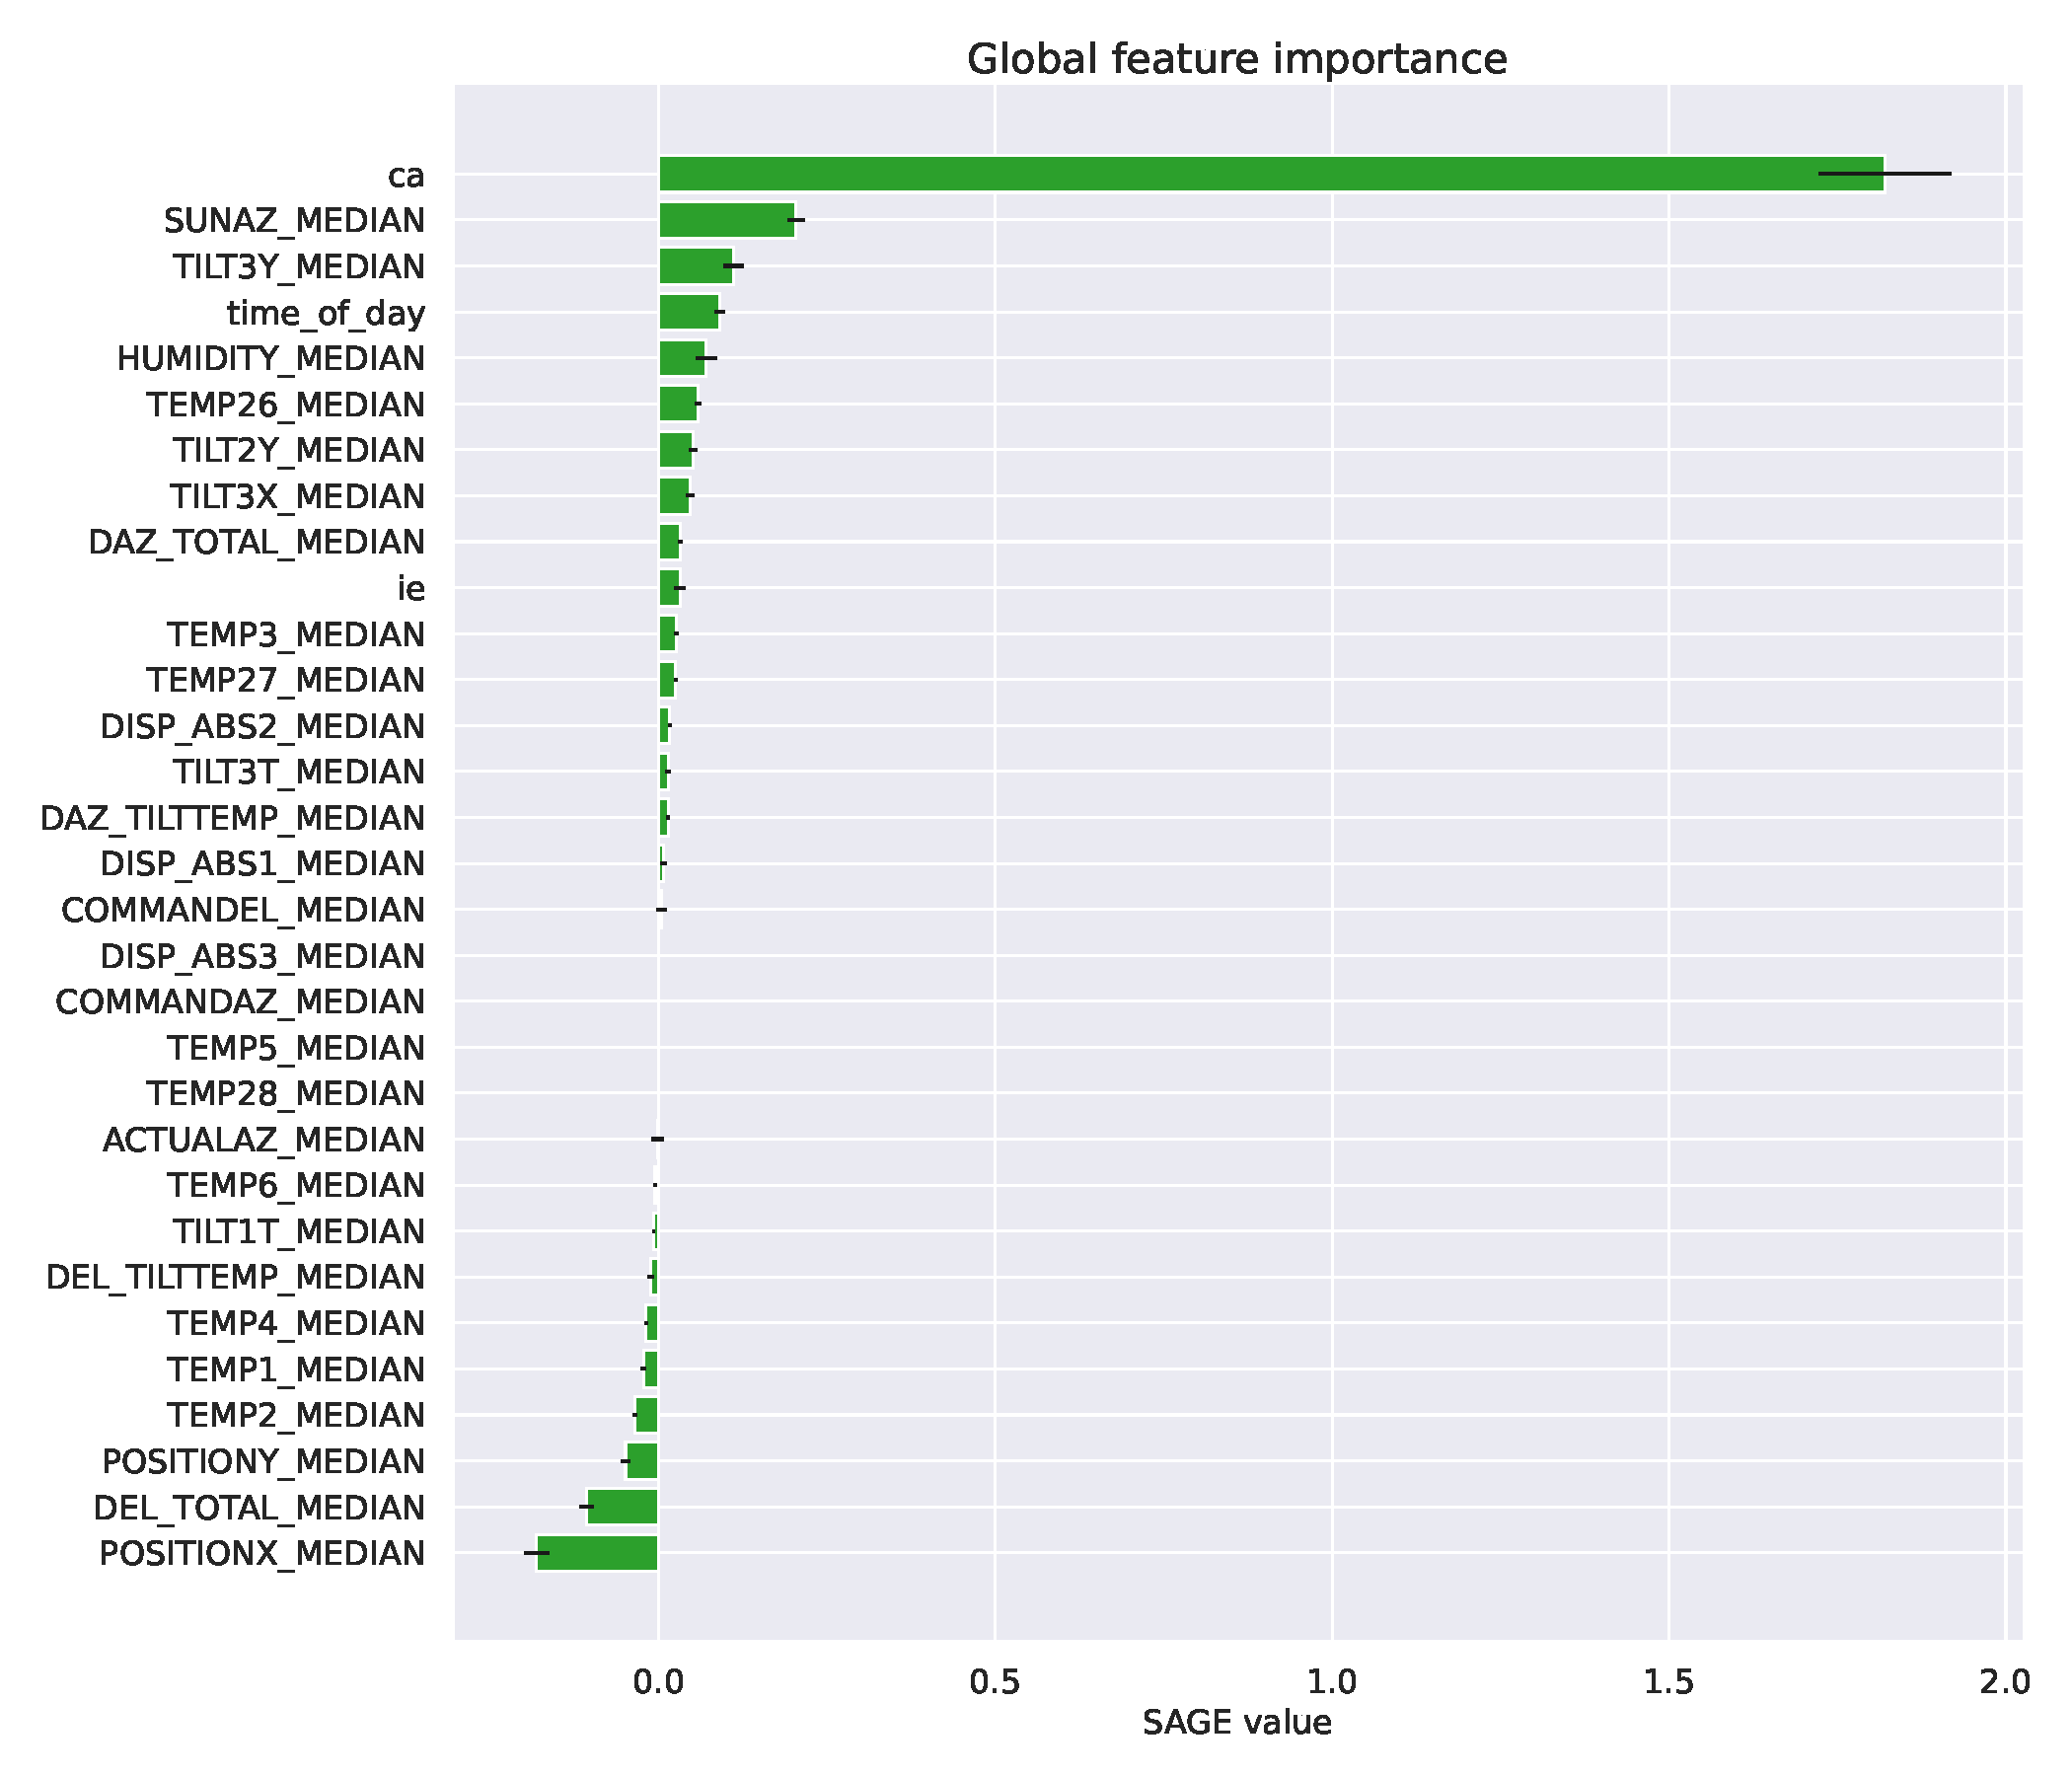
\includegraphics[width=1\textwidth]{Results/XGB_ds2_tp5_k30_uncorr_az_test_SAGE.pdf}
       \caption{Test set}
       \label{subfig:sage_lastfold_nflash230_az_test}
    \end{subfigure}
    \caption[SAGE values for NFLASH230 elevation pointing correction model]{SAGE values for the NFLASH230 azimuth pointing correction model on the a) validation set, and b) test set.}
    \label{fig:sage_lastfold_nflash230_az}
\end{figure}

\begin{figure}[H]
    \centering
    \begin{subfigure}[t]{0.92\textwidth}
        \centering
        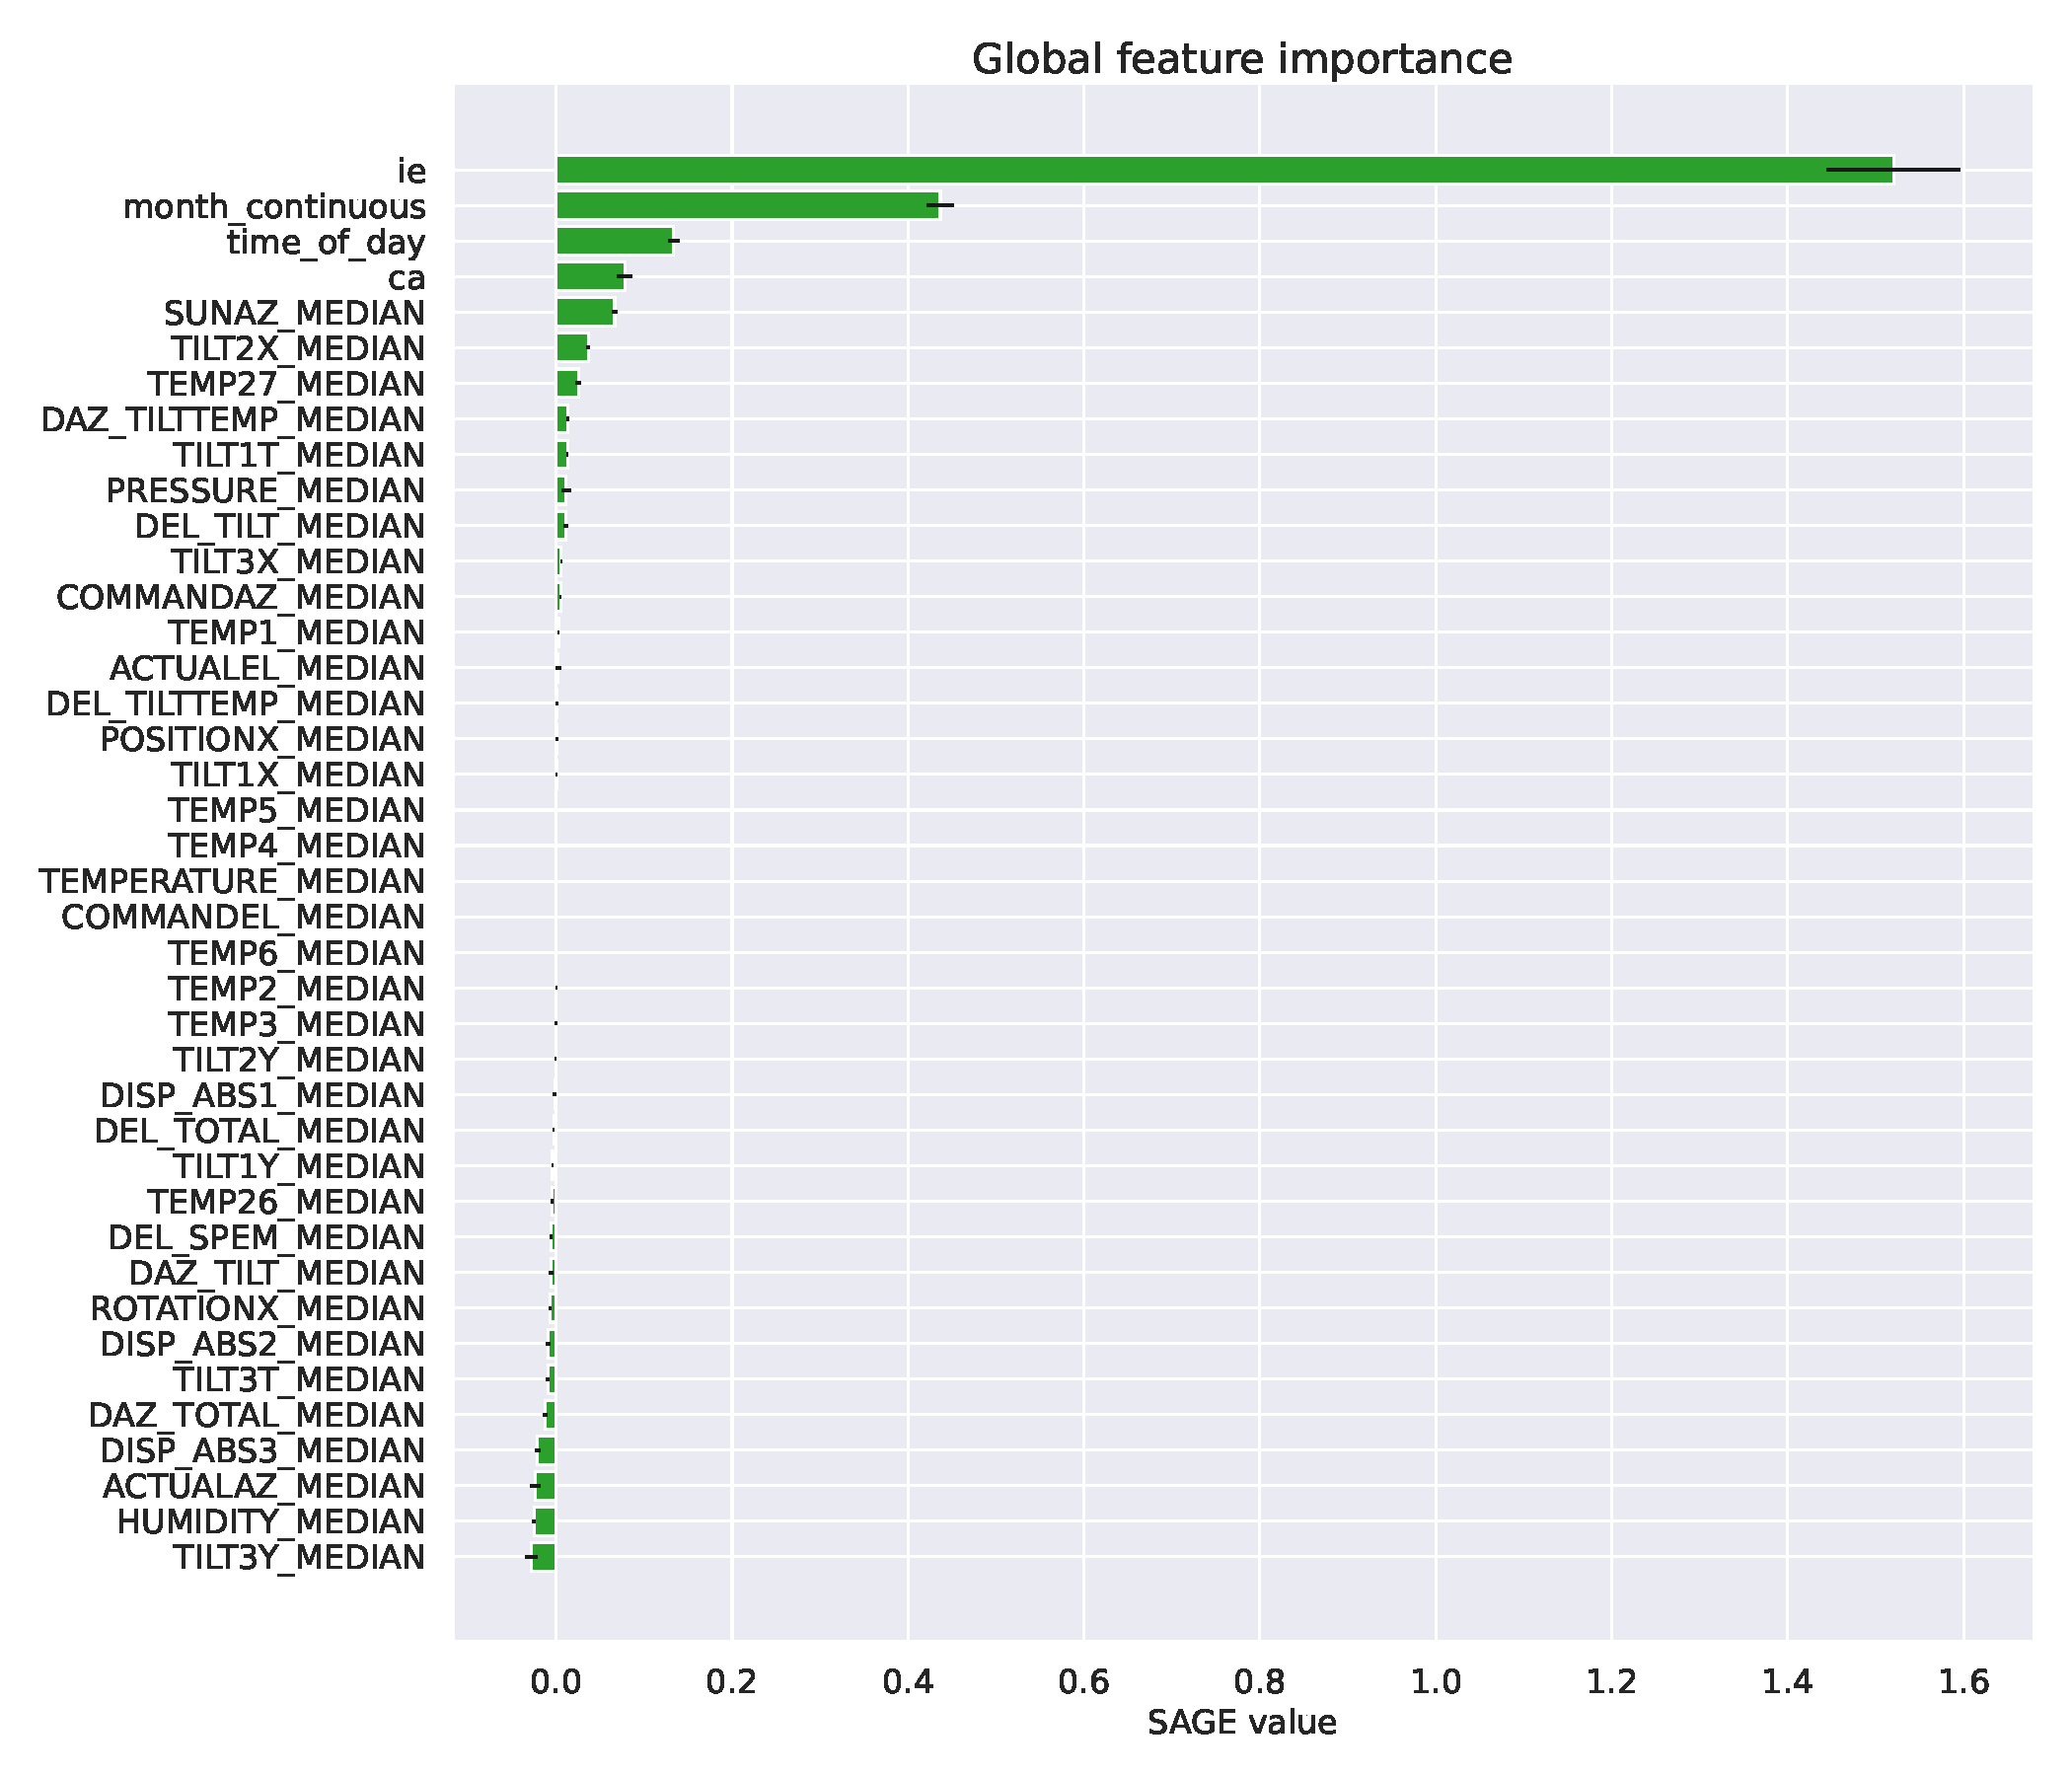
\includegraphics[width=\textwidth]{Results/XGB_ds2_tp5_k40_uncorr_el_val_SAGE.pdf}
        \caption{Validation set}
        \label{subfig:sage_lastfold_nflash230_el_val}
    \end{subfigure}
    \\
    \begin{subfigure}[t]{0.92\textwidth}
       \centering
       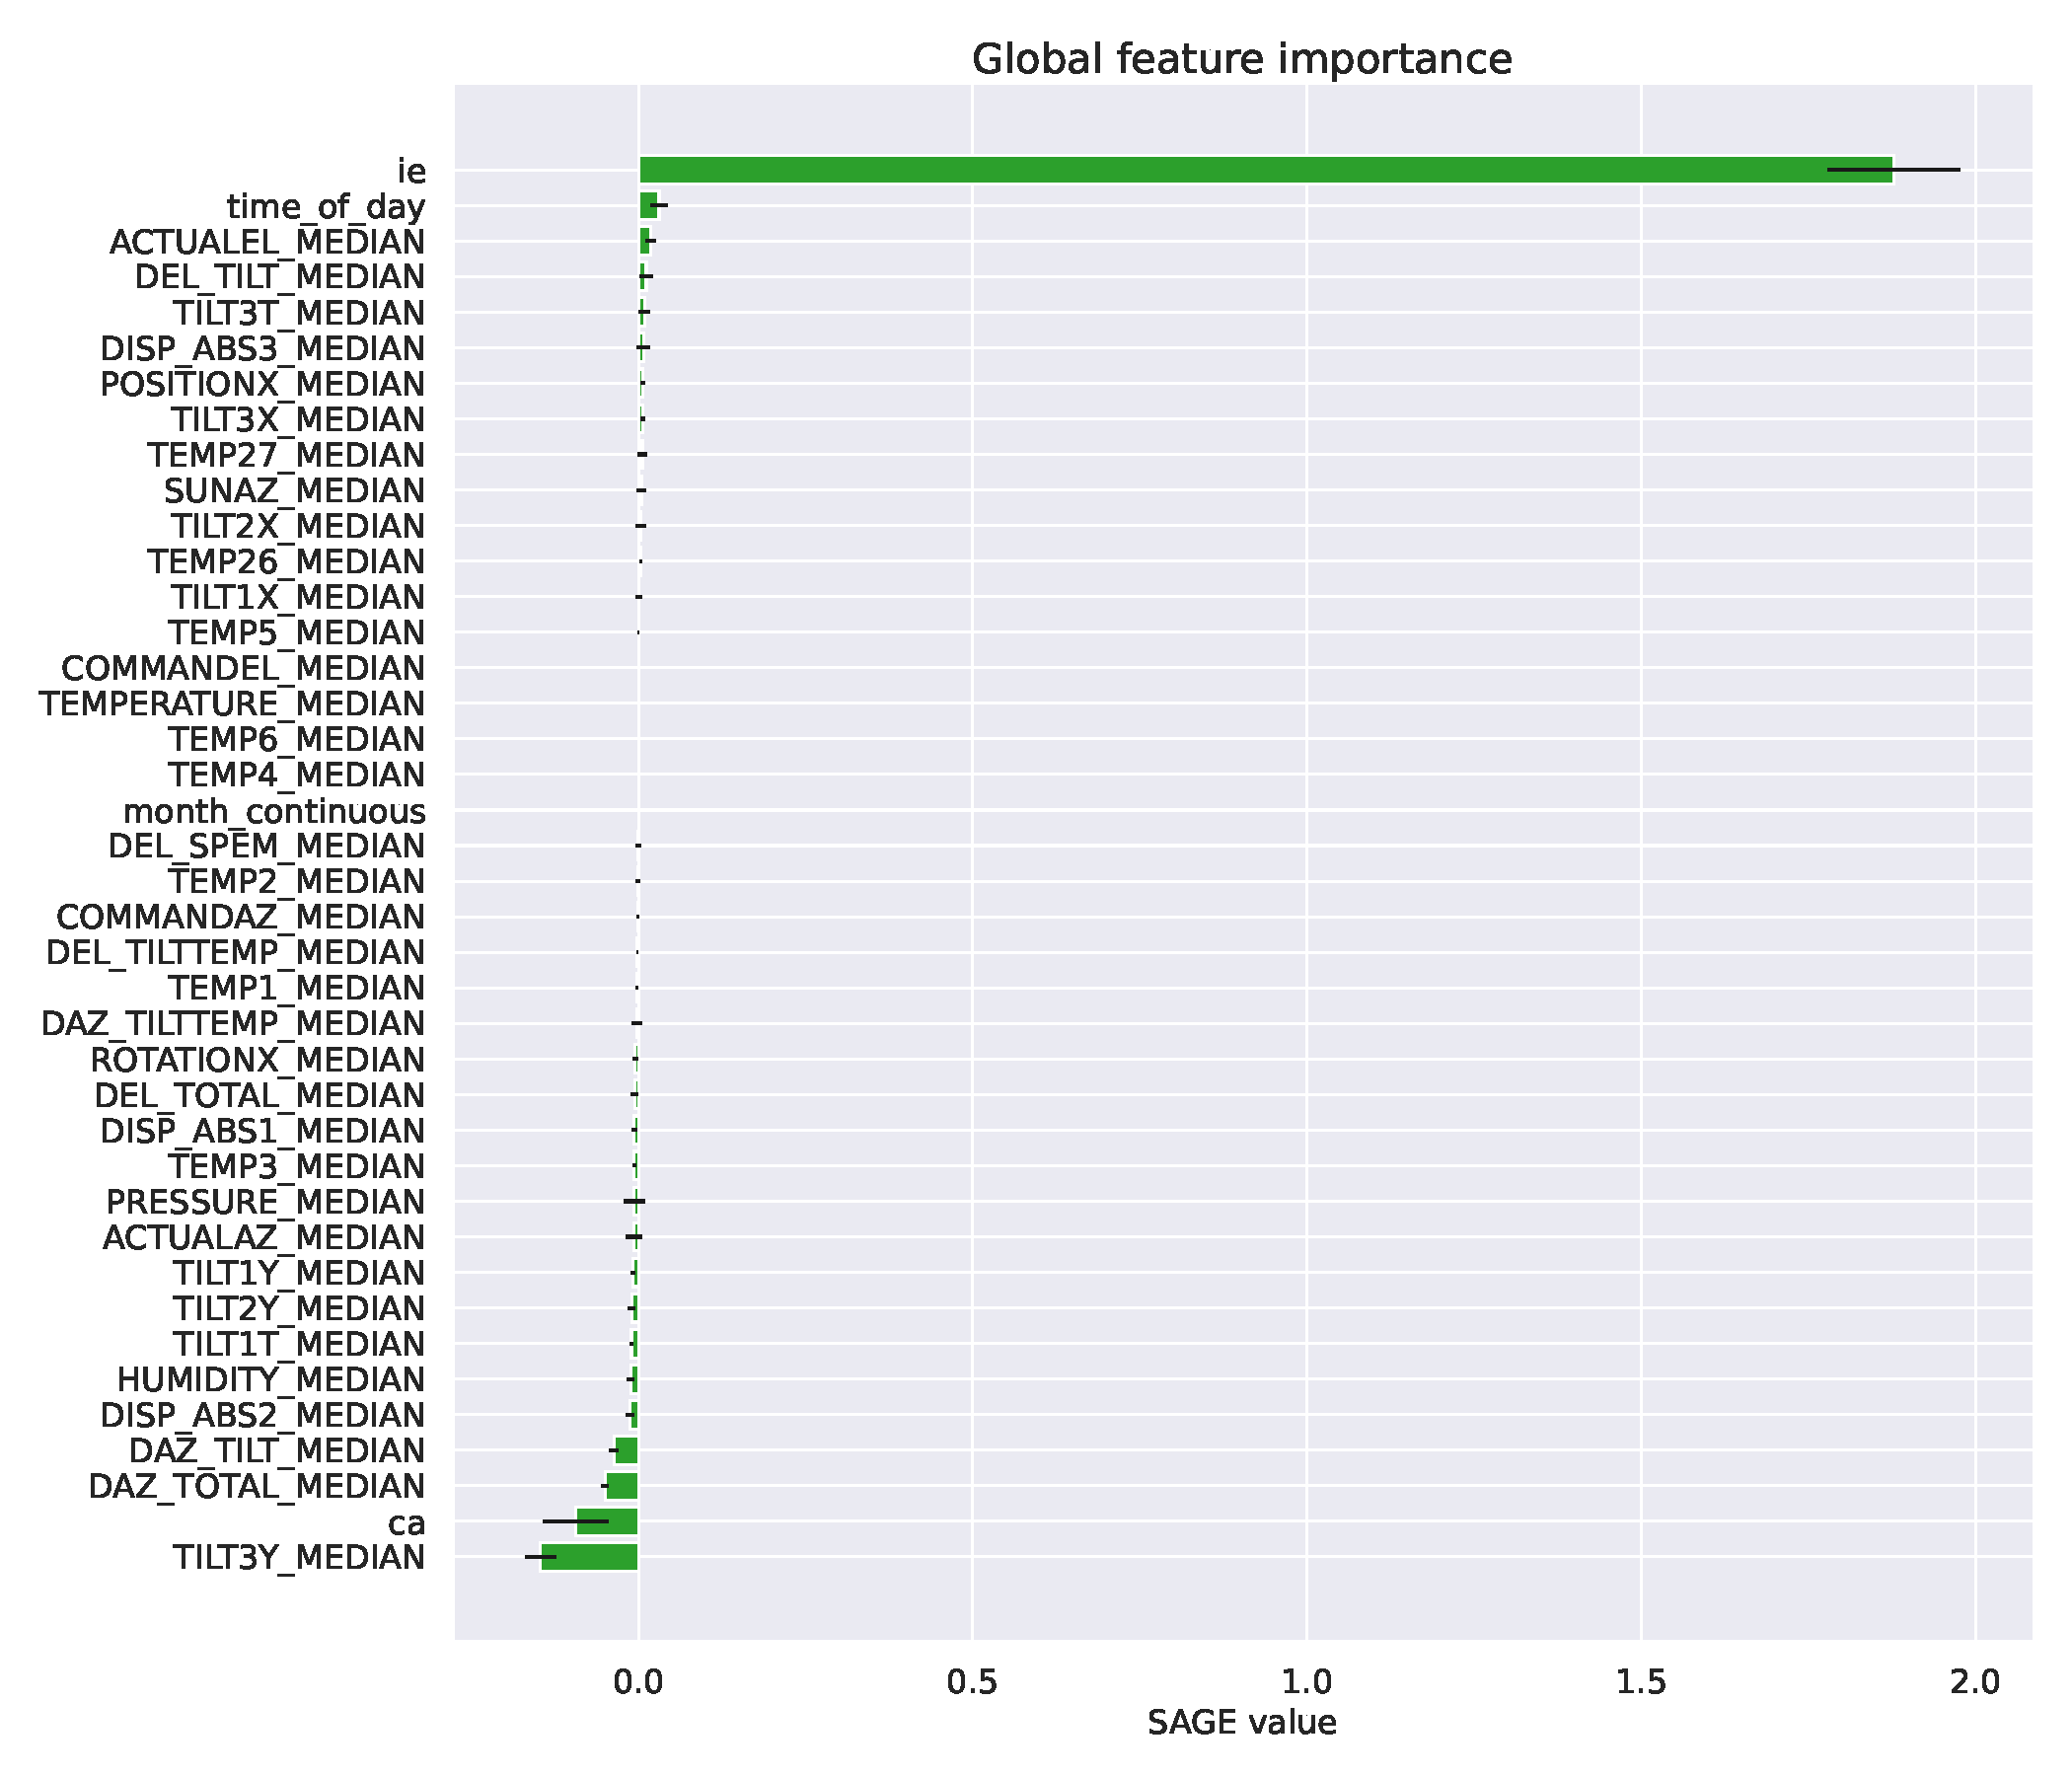
\includegraphics[width=1\textwidth]{Results/XGB_ds2_tp5_k40_uncorr_el_test_SAGE.pdf}
       \caption{Test set}
       \label{subfig:sage_lastfold_nflash230_el_test}
    \end{subfigure}
    \caption[SAGE values for NFLASH230 elevation pointing correction model]{SAGE values for the NFLASH230 elevation pointing correction model on the \textbf{a)} validation set, and \textbf{b)} test set.}
    \label{fig:sage_lastfold_nflash230_el}
\end{figure}


\section{Discussion of Experiment 1: Pointing Correction Model}
The first research question addressed in this thesis is whether machine learning can enhance the pointing accuracy of a radio telescope using the current pointing strategy.
To investigate this question, we explore a realistic scenario (case 1) in which a model is trained on a smaller period of data and used to predict the offset of consecutive scans for a period afterward.
We focus now on the model predicting the offsets of only NFLASH230.
The results from this case, presented in Table \ref{tab:results_minval_val_test_days_04_n230}, demonstrate that the model's performance on the validation set is promising,
with the root-mean-square (RMS) ratio in the range of approximately $0.80$-$0.85$ for azimuth and elevation,
which corresponds to a $15$-$20\%$ reduction in pointing offset.
However, this performance does not transfer to the following test period,
in which the RMS ratios are $1.16$-$1.46$, indicating a $16$-$46\%$ increase in pointing offset.
There are several possible reasons for the model's poor performance on the test set.
One of the limitations of tree-based models, such as XGBoost, is that they typically do not generalize well to new data that is different from the training data,
as they predict solely based on logical conditions seen in the training set.
If the factors affecting the pointing offset change over time and the new data is very different from the training data, the model will likely perform poorly. 
Furthermore, another potential explanation for the poor performance could be that the dataset is too small, and the model overfits on the validation set.
The results of this experiment suggest that learning the relationships in the data that affect pointing offset is challenging, and a complex model may be necessary.
To train a proper complex model, a larger amount of data is required, at least more than the number of samples in the training and validation sets for case 1.
The findings also indicate that choosing the complexity of the model with the best performance on the validation set may not necessarily lead to the best performance on the test set.
We further explore this aspect by examining Table \ref{tab:results_nflash_days}, which demonstrates the mean RMS ratio on the test set using the same number of features for all the folds.
This provides an idea of the complexity that might provide the best-performing models on the test set.
Even though the model with the best performance on the validation set is not chosen, which could be a lucky or overfitted performance,
no improvement is observed in the current pointing model on the test set.
However, the results show better performance than the first Table \ref{tab:results_minval_val_test_days_04_n230}.
The same trends are observed when predicting offsets from all instruments in Tables \ref{tab:results_minval_val_test_days_04_all} and \ref{tab:results_all_days}. \\


Moving on to case 2, which tests whether the amount of data is a limitation for enhancing the pointing accuracy.
This test case is less realistic because the data is split into $6$ folds and cross-validation is performed,
and for all folds except for the last one, the test period will be either before or between the training/validation set, making the results less applicable in practice.
Results from this case indicate that a larger time period helps the model generalize better, which is expected as a larger period includes more variation that can help the model capture the relationships between features.
We start by looking at the same table \ref{tab:results_minval_val_test_days_04_n230}.
Here, we also see a good performance on the validation set across all folds, with a $9$-$20\%$ reduced pointing offset on the validation set.
This shows that more training data helps the model generalize, which is somewhat expected considering that a larger time period includes more variation,
which helps the model learn what causes the offsets.
The average RMS ratio on all folds on the test set for case 2 is $0.958$ for azimuth and $0.941$ for elevation.
With the standard deviations, the $95\%$ confidence intervals would be put at $[0.850, 1.066]$ for azimuth and $[0.786, 1.010]$ for elevation.
Given that the upper bound of both confidence intervals is larger than one and the testing case is not realistic, we cannot conclude that the model can reduce the pointing offset robustly and consistently.
For an unbiased result that reflects expected performance in practice, we look at the RMS ratio for the last fold in Table \ref{tab:results_minval_val_test_days_04_n230},
showing a $7.0\%$ and $9.4\%$ reduced RMS for azimuth and elevation, respectively.
These results are the ones visualized in the histograms and plots in Figures \ref{fig:histogram_selected_result_xgb} and \ref{fig:sortpred_selected_result_xgb}, respectively.
It is not apparent from the histogram with the azimuth model results that the model performs better than the current model.
What we can see, however, is a shift in offsets towards the left, indicating more negative offsets.
This is consistent with the sorted prediction plot \ref{subfig:sortpred_lastfold_nflash230_az}, which shows a bias towards positive predictions.
There also seem to be slightly less large negative offsets.
Looking at the elevation histogram \ref{subfig:hist_lastfold_nflash230_el} and plot \ref{subfig:sortpred_lastfold_nflash230_el}, we can make the same analysis.
The histogram shows a shift towards the left, and the sorted prediction plot shows a bias toward positive predictions.
We do also see that there are more offsets in the center bin in the histogram (meaning more smaller offsets).
The tails in the sorted prediction plots also seem steep, indicating that the cleaning could have been better.\\


We now discuss the results of the SAGE analysis on the validation and test sets for the model discussed in the previous paragraph,
as shown in Figures \ref{fig:sage_lastfold_nflash230_az} and \ref{fig:sage_lastfold_nflash230_el}.
This analysis helps us understand the factors that improve and worsen the models' performance on unseen data, thereby providing insights into how the models can be improved.

For the azimuth model, we observe that the azimuth correction $ca$ is the most important feature, contributing significantly to the model's performance on both the validation and test sets.
However, the elevation correction $ie$ shows a mixed effect on the model's performance.
While it improves the performance on the validation set, it worsens the performance on the test set.
This indicates that there are some correlation between the azimuth and elevation correction that change over time.
% Surprisingly, some features such as the azimuth angle of the sun and the $X$ position of the subreflector (POSITIONX) worsen the performance on the validation set, but improve it on the test set.
% We do not have a clear explanation for this behavior.
Notably, the COMMANDAZ and COMMANDEL features, which are included in every model, do not affect the azimuth or elevation model's performance.
This suggests that the analytical pointing model, which is based solely on azimuth and elevation, is performing very well, and the sources of offsets are likely attributed to factors other than the pointing direction.
We also find that the continuous month feature is the second most important feature in the elevation model, after the elevation correction $ie$.
However, the model's performance on the test set does not benefit from this feature, as its value is larger in the test set than in the training and validation sets.
This is one of the weaknesses of tree-based models.
Training the model on the previous years' data could solve this problem, as long as there are not other big changes in the structure or mounting of the instruments.

% We now look at the results from the SAGE analysis on the validation and test set, shown in Figures \ref{fig:sage_lastfold_nflash230_az} and \ref{fig:sage_lastfold_nflash230_el},
% for the same model we discussed in the previous paragraph.
% Analyzing which features improve and worsen the performance on unseen data is a good way of understanding what makes the model better and worse.
% We start by looking at the sage values for the azimuth model \ref{fig:sage_lastfold_nflash230_az}.
% It shows that the azimuth correction $ca$ applied during the given pointing scan stands for most of the good predictions on both the validation and test set.
% The elevation correction $ie$ improves the performance on the validation set, but worsen the performance on new data.
% Interestingly enough, there are features like the azimuth angle of the sun and x position of the subreflector that makes the performance on the validation set worse, but improve the performance on the test set.
% We cannot explain this behavior either.
% Interestingly enough, COMMANDAZ and COMMANDEL, which is incorporated in every model, does not affect the performance of the model at all.
% This indicates that the analytical pointing model, which is only based on azimuth and elevation, is performing very well,
% and the reasons for the offsets are attributed to other factors.
% One interesting note, is that the continuous month feature in the elevation model is the second most important feature, after the elevation fcorrection $ie$.
% However, on the test set, the month continuous variable does not help the model at all.
% This is very expected behavior, as this value is larger on all the pointing scans in the test set, and therefore it cannot help the model,
% as there is nothing trained on the month being larger than it is in the training and validation set.
% Again here, we see taht the input coordinates are of no use for the model.



In summary of the results from case 2, we see promising results with machine learning models further reducing the offsets slightly.  
This indicates that a possible pointing strategy could be training a model on multiple months worth of data and then using the model for a couple of weeks.
However, given the limited data available in this project, this could not be tested thoroughly.
If more data were available,
a similar analysis could be performed with the start and end time of both the train/validation and test set moved by two weeks and iteratively train new models to predict the offsets for the next time period.
This could verify whether the improved performance repeats.\\



In case 2, the model predicting offsets from all instruments shows results similar to the model predicting only NFLASH230 offsets, though with slightly worse performance.
The reduced performance is likely due to less training data available for the other instruments.
The difference in performance between these two models provides some insights.
First, it suggests that various factors influence the different instruments differently.
Otherwise, we expect the larger model to perform better than the smaller model.
The reason that each instrument can be affected differently is because of the different mounting locations at the telescope.
Different mounting locations mean that the path of photons leading to the receiver can vary, leading to distinct factors affecting the pointing.\\


There are several measures we could take to enhance the analysis further. One such measure is to improve feature engineering.
When the quantity of training data is limited, it is vital to ensure that the features are as informative as possible.
For example, instead of including six distinct temperature measurements in a model,
it may be preferable to create terms based on the difference between multiple temperature measurements, as they did in \cite{whitegreen2022}.

Another step is to integrate corrections for $ca$ and $ie$ into the offset that we intend to predict.
These corrections are applied at each pointing scan and display the strongest correlation to the target offset of all the features,
and we, therefore, incorporate them in all the models.
By transforming the offsets $\delta_{az}=\delta_{az} + ca$ and $\delta_{el}=\delta_{el} + ie$, we can then eliminate $ca$ and $ie$ from the input to the models.
This could remove a layer of complexity for the model.\\


Another option to consider for predicting the pointing offsets is to use neural networks.
These models offer several advantages if trained successfully.
For instance, they can handle multiple outputs and thus only require a single model.
By training the neural network with two outputs, it can simultaneously consider the offsets in azimuth and elevation and explore the correlation between them.
It would also be beneficial to fine-tune the network as new pointing scans become available continuously.
Despite their potential benefits, our initial tests with neural networks did not yield satisfactory results,
likely due to the limited training data available. Neural networks also require more tuning, which makes them more difficult to use with limited datasets.\\


To further improve the analysis, there are other possible areas for exploration, such as minimizing the number of pointing scans conducted by the astronomers.
While performing scans every one to two hours is standard practice, this can be time-consuming and may disrupt science observations.
A possible approach to investigate this possibility is to identify periods when pointing scans are conducted every hour or so.
Rather than providing the model with the corrections $ca$ and $ie$ obtained following the previous pointing scan, the model can be fed with the corrections from a pointing scan that occurred six hours earlier to evaluate its performance.
In this case, reducing pointing offsets is not a primary objective of the machine learning approach.
Instead, maintaining the same level of pointing accuracy while conducting fewer pointing scans would be a satisfactory outcome.\\



% \begin{itemize}
%     \item comment on parameters
%     \item discuss the adjustments made by system,a nd that the analytical poinitng models change over time too, which can make it harder for amodel, considering there are many other factors to ocnsider.
% \end{itemize}

% \section{Experiment 2: Pointing Correction Model}
% The first research question is if we can use machine learning to increase the pointing accuracy using the same pointing strategy as today.
% We start by discussing case 1, which test a realistic scenario of training a model on a smaller period,
% and then using the model to predict the offset of the consecutive scans for a period.
% We look first at the model using NFLASH230 data only.
% The results from this case show that the performance on the validation set is good \ref{tab:results_minval_val_test_days_04_n230},
% with the RMS ratio being in the range $\tilde{}0.80$-$0.85$ for azimuth and elevation.
% That corresponds to a $15$-$20\%$ reduced pointing offset.
% This performance does not transfer to the following test period,
% for which the RMS ratios are in the range $1.16$-$1.46$, corresponding to a $16$-$46\%$ increased pointing offset.
% There could be multiple reasons for the drastically worse performance set.
% One possibility is that the relationships learned by the model change over time, therefore the model is not able to perform well.
% This is one limitation of tree based models like XGBoost.
% Because the model is predicting solely on logical conditions seen in the training set,
% it is not able to generalize well to new data.
% A neural network could potentially perform better on unseen data, as it train a continuous function.
% Another reason is that the dataset is too small, and the performance on the validation set is based on luck.
% In other words, model overfits on the validation set.
% From this project, it is clear that learning the relationships in the data that affects the pointing offset is not easy, and a complex model might be essential.
% And in order to train a proper complex model, we need large amounts of data,
% at least more than the \textcolor{red}{train set num} and \textcolor{red}{train set num} samples in the training and validation set respectively.
% The resutls we just discussed, uses a strategy where we choose the complexity of the model with the best performance on the validation set.
% We now look at Table \ref{tab:results_nflash_days}, which shows the mean RMS ratio on the test set using the same number of features $k$ for all the folds.
% This gives an idea on what complexity could provide the best models.
% It shows that even though we do not choose the model with the best performance on the validation set, which could potentionally be a lucky performance or overfitted,
% we still do not see any improvement of the current pointing model on the test set.
% We do however see better results than in the first table \ref{tab:results_minval_val_test_days_04_n230}.
% If we look at the model using the data from all instruments, we see similar results \ref{tab:results_minval_val_test_days_04_all} \ref{tab:results_all_days}.\\

% Now onto case 2, which show a less realistic test case, but can give an idea on if the amount of data is a limitation.
% This test case is less realistic because we split the data into $6$ folds and perform cross validation.
% For all folds except for the last one, the test period will be either before, or between the training/validation set.
% Therefore, these results does not reflect expected performance in practise.
% We start by looking at the same table \ref{tab:results_minval_val_test_days_04_n230},
% with results from the NFLASH230 model choosing the best model from the validation set, and tests the performance on the test set.
% Again, we see a good performance on the validation set across all folds, with a $9$-$20\%$ reduced pointing offset, for azimuth and elevation models.
% Now, we also see a reduced pointing offset even on the test set.
% This shows that more training data helps the model generalize,
% which is somewhat expected considering that a larger time period includes more variation, which helps the model capture relations between features.
% The average RMS ratio on all folds for case 2 is $0.958$ for azimuth and $0.941$ for elevation.
% With the standard deviations, the $95\%$ confidence intervals would be put at $[0.850, 1.066]$ for azimuth and $[0.786, 1.010]$ for elevation.
% The results show that there is something to be learnt in the data, and this pointing strategy could potentially lead to improved pointing.
% For a completely unbiased result, which show a performance that could have been achieved in practice,
% we look at the RMS ratio for the last fold in Table \ref{tab:results_minval_val_test_days_04_n230}.
% This shows a $7.0\%$ and $9.4\%$ reduced RMS for azimuth and elevation respectively,
% which indicates that a possible pointing strategy could be training a model on multiple months worth of data, and then use the model for a couple of weeks.
% Given we only have six months of data, this could not be tested more thoroughly.
% If we had more data, we could trained a model on the same amount of data, but moving the start and end time of both the train/validation and test set by two weeks, and
% see if the improved performance repeats.




% \begin{align}
%     CI_{Az} &= \bar{r}_{RMS_Az} \pm 1.96 \cdot \sigma_Az = [0.958 - 1.96\cdot 0.055, 0.958 + 1.96\cdot 0.055] = [0.850, 1.066]  \\
%     CI_{El} &= \bar{r}_{RMS_El} \pm 1.96 \cdot \sigma_El = [0.941 - 1.96\cdot 0.079, 0.941 + 1.96\cdot 0.079] = [0.786, 1.010]
% \end{align}


\section{Results of Experiment 2: Pointing Model using Neural Networks}

Table \ref{tab:exp1_rms_folds_best_model} shows the RMS in arcseconds on the test set overall folds for the different model architectures.
The models presented in this table are the ones with the lowest mean RMS across all test folds.
A linear regression model is included for comparison. 
It is clear that neural network architectures significantly outperform the linear regression model.
From the mean RMS overall folds, we see that the different neural network architectures offer similar performance.
We also see that the RMS of fold $1$ is by far worse than the other folds.
The lowest mean RMS is from the architecture where the non-linear features are connected to the geometrical and harmonic features.\\

\begin{table}[!htbp]
    \centering
    \caption[RMS of each pointing model architecture on all test folds]{The RMS of the pointing model on the test set in each fold for all neural network architectures.
    The different architectures are described in Figure \ref{fig:nn_architecture}.}
    \begin{tabular}{lcccccccc}
        \toprule
        & \multicolumn{6}{c}{RMS [$''$] on test fold} & & \\
        \cmidrule(lr){2-7}
        Network & 1 & 2 & 3 & 4 & 5 & 6 & Mean & STD\\
        \midrule
        Regular           & 28.06 & 19.34 & 12.28 & 13.25 & 17.19 & 16.33 & 17.74 & 5.19 \\
        Separated 1       & 30.69 & 16.93 & 13.76 & 10.04 & 15.77 & 13.61 & 16.80 & 6.57 \\
        Separated 2       & 27.34 & 20.75 & 12.65 & 24.17 & 13.64 & 16.69 & 19.21 & 5.38 \\
        Separated 3       & 30.27 & 20.59 & 14.01 & 10.76 & 13.67 & 10.34 & 16.61 & 6.97 \\
        Linear regression & 70.55 & 40.19 & 51.17 & 49.69 & 36.86 & 37.29 & 47.63 & 12.81 \\
        \bottomrule
    \end{tabular}
    \label{tab:exp1_rms_folds_best_model}
\end{table}


Table \ref{tab:exp1_hyperparameters_best_model} shows the hyperparameter used for the best models.
All architectures perform better with a single hidden layer.
The regular neural network uses ReLU activation and MSE loss, while the other architectures use Tanh activation and MSD loss.
The regular neural network also has more neurons in the hidden layer and a higher learning rate.
The batch size is also varying. There seem to be similarities between the hyperparameters chosen for the three architectures with separate features.
However, given the large standard deviation of the mean RMS, there are probably bigger issues than hyperparameter tuning.\\

\begin{table}[!htbp]
    \centering
    \caption[Selected hyperparameters for each neural network pointing model architecture]{Hyperparameters used in the best-performing model for each architecture.}
    \begin{tabular}{lccccc}
        \toprule
        Architecture & Activation & Hidden Layers & Learning Rate & Batch Size & Loss \\
        \midrule
        Regular &  ReLU & [82] & 0.0199 & 334 & MSE \\
        Sep1    &  Tanh & [40] & 0.0098 & 101 & MSD \\
        Sep2    &  Tanh & [40] & 0.0098 & 101 & MSD \\
        Sep3    &  Tanh & [26] & 0.0039 & 358 & MSD \\
        \bottomrule
    \end{tabular}
    \label{tab:exp1_hyperparameters_best_model}
\end{table}



Table \ref{tab:exp1_features} lists the features selected for the best-performing models.


\begin{table}[!htbp]
    \centering
    \caption[Selected features for each neural network pointing model architecture]{Features used in the best-performing model for each architecture.}
    \begin{tabular}{|l|ccccc|}
        \hline
        Feature & Sep 1 & Sep 2 & Sep 3 & Regular & \\ \hline
        COMMANDAZ & x & x & x & x & \\ \hline
        COMMANDEL & x & x & x & x & \\ \hline
        DISP ABS3 & x & x & x & x & \\ \hline
        CA & x & x & x & & \\ \hline
        NPAE & x & x & x & & \\ \hline
        Constant & x & x & x & & \\ \hline
        $\cos{(\text{COMMANDEL})}$ & x & x & x & & \\ \hline
        $\cos{(2\cdot \text{COMMANDEL})}$ & x & x & x & & \\ \hline
        $\cos{(3\cdot \text{COMMANDEL})}$ & x & x & x & & \\ \hline
        $\cos{(4\cdot \text{COMMANDEL})}$ & x & x & x & & \\ \hline
        $\cos{(5\cdot \text{COMMANDEL})}$ & x & x & x & & \\ \hline
        $\sin{(\text{COMMANDEL})}$ & x & x & x & & \\ \hline
        $\sin{(2 \cdot \text{COMMANDEL})}$ & x & x & x & & \\ \hline
        $\sin{(3 \cdot \text{COMMANDEL})}$ & x & x & x & & \\ \hline
        $\sin{(4 \cdot \text{COMMANDEL})}$ & x & x & x & & \\ \hline
        $\sin{(5 \cdot \text{COMMANDEL})}$ & x & x & x & & \\ \hline
        Turbulence & x & x & x & & \\ \hline
        DEL TILTTEMP & x & x & x & & \\ \hline
        DAZ DISP & & & x & & \\ \hline
        POSITIONY & & & x & & \\ \hline
        TILT1Y & & & x & & \\ \hline
        TEMPERATURE & & & x & & \\ \hline
        TILT1T & & & x & & \\ \hline
    \end{tabular}
    \label{tab:exp1_features}
\end{table}


\section{Discussion of Experiment 2: Pointing Model using Neural Networks}

To address the second research question of whether machine learning models can replace the traditional analytical linear regression models commonly used in radio/(sub-)mm telescopes,
we utilized raw data from the apex telescope containing input and observed coordinates for azimuth and elevation.
Typically, linear regression models are fitted to this raw data using multiple geometrical and empirical terms.
As a benchmark, we used a linear regression model and compared its performance against four different neural network architectures (see Figure \ref{fig:nn_architecture}).
Our goal was to determine if a machine learning approach could outperform the linear regression model and, if so, which type of architecture performs the best.
We employed cross-validation with six folds and found that all neural network architectures significantly outperformed the linear regression model.
The mean RMS of the linear regression model was $47.63''$ with a standard deviation of $12.81''$, whereas all neural network architectures fell within the range of $16''$-$19''$ with deviations of $5''$-$7''$.
Although all the neural network architectures had similar performance and standard deviation, we cannot conclude that any of them is better than the others.
Overall, our results indicate that machine learning models can outperform traditional analytical models for pointing offset prediction in radio telescopes,
and we encourage further research in this area to explore the full potential of machine learning techniques.\\

Analysis of the hyperparameters selected for the top-performing models reveals that most of them are relatively simple in structure.
Interestingly, none of the models employed two hidden layers.
Additionally, the architectures incorporating distinct layers for the terms employed in the analytical pointing models exhibited lower neuron counts in their nonlinear layers.
This is likely because the level of complexity required for the input features provided to the nonlinear layers is assumed to be lower when other aspects of the model are responsible for handling certain factors.
Thus, the observed pattern of hyperparameter selection is consistent with the expectation based on architecture.\\

Table \ref{tab:exp1_features} presents the features selected by each model.
All the models included COMMANDAZ and COMMANDEL as inputs for the nonlinear layers.
The "Separated" neural networks incorporated the harmonic features as inputs in the linear part of the network, shown in Figure \ref{fig:nn_architecture}.
We sampled the remaining features randomly.
Interestingly, the models used few nonlinear features, indicating that the factors influencing pointing error are difficult to model with the current training set.
Obtaining more data may be necessary to establish more complex relationships between features that can improve the performance of the pointing models.
Notably, the regular neural network utilized only one additional feature, namely DISP\_ABS (which still requires explanation).
This finding suggests that a neural network utilizing only the azimuth and elevation angle could outperform a linear regression model.
However, linear regression models have advantages in terms of transparency and robustness, as they are inherently linear, and all the features in the model are independent of each other,
resulting in a model that is unlikely to result in significant pointing errors.
This is an important consideration when using machine learning models, which can be challenging to interpret.
Their robustness must be thoroughly tested before being deployed in practical settings.
These considerations also underlie the design of the "Separated" neural network architectures.
We wanted to utilize the robustness of linear regression on the terms used in the current analytical pointing model while incorporating new features. 
Considering that the experiment demonstrated negligible performance differences between the separate neural networks and the regular
one and that the best models only choose a few features, we conclude that additional training data is required to see if this is a feasible approach.\\

While the experiment did not demonstrate the performance that would be expected from using such models in practice,
it indicates that a neural network could provide a more efficient and effective model than a linear regression model.
Moreover, a neural network can be fine-tuned with newly obtained data, making it an appealing model.
If this approach is shown to be reliable and high-performing, it could be the preferred choice for more advanced telescopes, as it may require less manual analysis to develop and maintain a pointing model.
However, further testing with additional data is needed to confirm the feasibility of this approach.
